% -------------------------------
% --- PREAMBLE ---
% -------------------------------
\documentclass[a4paper,11pt]{article}
\usepackage[utf8]{inputenc}



\usepackage{amsmath,amssymb,amsfonts,amsthm}    % Typical maths resource packages
\usepackage{graphicx}                           % Packages to allow inclusion of graphics
%\usepackage[authoryear]{natbib}                 % literature reference style
\usepackage{natbib}
\usepackage[bf]{caption}
\usepackage{textcomp}                           % For single quotes
\usepackage{floatrow}                           % For image and table position
\usepackage{booktabs}                           % For tables
\usepackage[hidelinks]{hyperref}
% \usepackage[colorlinks=true]{hyperref}                           
% \usepackage[bottom]{footmisc}                   
\usepackage[bottom, flushmargin]{footmisc}                   % For footnotes
%\usepackage[citebordercolor={0 1 0}]{hyperref}                           % For creating hyperlinks in cross references
\usepackage{footnotebackref}

% From {rticles}
\newlength{\csllabelwidth}
\setlength{\csllabelwidth}{3em}
\newlength{\cslhangindent}
\setlength{\cslhangindent}{1.5em}
% for Pandoc 2.8 to 2.10.1
\newenvironment{cslreferences}%
  {}%
  {\par}
% For Pandoc 2.11+
% As noted by @mirh [2] is needed instead of [3] for 2.12
\newenvironment{CSLReferences}[2] % #1 hanging-ident, #2 entry spacing
 {% don't indent paragraphs
  \setlength{\parindent}{0pt}
  % turn on hanging indent if param 1 is 1
  \ifodd #1 \everypar{\setlength{\hangindent}{\cslhangindent}}\ignorespaces\fi
  % set entry spacing
  \ifnum #2 > 0
  \setlength{\parskip}{#2\baselineskip}
  \fi
 }%
 {}
\usepackage{calc} % for calculating minipage widths
\newcommand{\CSLBlock}[1]{#1\hfill\break}
\newcommand{\CSLLeftMargin}[1]{\parbox[t]{\csllabelwidth}{#1}}
\newcommand{\CSLRightInline}[1]{\parbox[t]{\linewidth - \csllabelwidth}{#1}}
\newcommand{\CSLIndent}[1]{\hspace{\cslhangindent}#1}


% -------------------------------
% --- some layout definitions ---
% -------------------------------

% define topline
\usepackage[automark]{scrlayer-scrpage}
\pagestyle{scrheadings}
\automark{section}
\clearscrheadings
\ohead{\headmark}

% define citation style
\bibliographystyle{apalike}

% define page size, margin size
\setlength{\headheight}{1.1\baselineskip}
\voffset=-2cm
\hoffset=-3cm
\textheight24cm
\textwidth15.5cm
\topmargin1cm
\oddsidemargin3cm
\evensidemargin3cm
\setcounter{secnumdepth}{3}
\setcounter{tocdepth}{3}   
  \usepackage[parfill]{parskip} 

% define line spacing = 1.5
\renewcommand{\baselinestretch}{1.5}

% define position of graphics
\floatsetup[figure]{capposition=bottom}
\floatsetup[table]{capposition=bottom}
\floatplacement{figure}{tb}
\floatplacement{table}{tb}

% save thesis parameters for later
\newcommand{\thesisauthor}{Rikard Wahlström}
\newcommand{\thesisdate}{}

% define tightlist to work with newer versions of pandoc
\providecommand{\tightlist}{%
  \setlength{\itemsep}{0pt}\setlength{\parskip}{0pt}}

% change spacing
\setlength {\parskip}{1em}

% Additional LaTeX parameters added in the YAML header of index.Rmd

% --------------------------------------
% --------------------------------------
% --------------------------------------
% --- the structure the tex document ---
% ---  (this our recommendation) -------
% frontmatter:
%   - titlepage (mandatory),
%   - acknowledgement,
%   - abstract,
%   - table of contents (mandatory),
%   - list of abbreviations (not mandatory),
%   - list of figures (not mandatory),
%   - list of tables  (not mandatory) .
%
% body of the thesis (the structure of the thesis body is not mandatory, but the list of literature is mandatory):
%   - introduction,
%   - methods,
%   - data,
%   - results,
%   - conclusion,
%   - literature (mandatory),
%   - appendix (figures, tables).
%
% last page:
%   - declaration of authorship (mandatory).
% --------------------------------------
% --------------------------------------
% --------------------------------------

\usepackage{amsthm}
\newtheorem{theorem}{Theorem}[section]
\newtheorem{lemma}{Lemma}[section]
\newtheorem{corollary}{Corollary}[section]
\newtheorem{proposition}{Proposition}[section]
\newtheorem{conjecture}{Conjecture}[section]
\theoremstyle{definition}
\newtheorem{definition}{Definition}[section]
\theoremstyle{definition}
\newtheorem{example}{Example}[section]
\theoremstyle{definition}
\newtheorem{exercise}{Exercise}[section]
\theoremstyle{definition}
\newtheorem{hypothesis}{Hypothesis}[section]
\theoremstyle{remark}
\newtheorem*{remark}{Remark}
\newtheorem*{solution}{Solution}
\begin{document}
% -------------------------------
% --- frontmatter: Swedish title page ---
% -------------------------------

% -------------------------------
% --- frontmatter: English title page ---
% -------------------------------
\thispagestyle{empty}
\begin{center}

\includegraphics[width=7cm]{UU_logo_CMYK.eps}
\end{center}
\vspace{1.5cm}
\begin{center}
\begin{Large}
{\bf Estimating expected shortfall using an unconditional peaks-over-threshold method under an extreme value approach} 
\end{Large}
\end{center}
\vskip1.5cm
\renewcommand{\baselinestretch}{1}
\begin{center}
{\large Rikard Wahlström} 
\vskip2.5cm
\begin{center}
\begin{large}
{\it Bachelor's thesis in Statistics}\\
\end{large}
\end{center}
\vskip2cm
{\large\it Advisor}\\
{\large Lars Forsberg} 
\vskip2cm
{\large Spring 2021} 
\end{center}\vfill

% ------------------------------------
% --- frontmatter: Acknowledgement ---
% ------------------------------------
\pagestyle{plain}
\pagenumbering{roman}   % define page number in roman style
\setcounter{page}{1}    % start page numbering

% -----------------------------
% --- frontmatter: Abstract ---
% -----------------------------
\newpage
\hypertarget{abstract}{%
\section*{Abstract}\label{abstract}}
\addcontentsline{toc}{section}{Abstract}

Value-at-Risk (VaR) has long been the standard risk measure in financial risk management. However, VaR suffers from critical shortcomings as a risk measure when it comes to quantifying the most severe risks, which was made especially apparent during the financial crisis of 2007--2008. An alternative risk measure addressing the shortcomings of VaR known as expected shortfall (ES) is gaining popularity and is set to replace VaR as the standard measure of financial risk.

This thesis introduces how extreme value theory can be applied in estimating ES using an unconditional peaks-over-threshold method. This includes giving an introduction to the theoretical foundations of the method. An application of this method is also performed on five different assets. These assets are chosen to serve as a proxy for the more broad asset classes of equity, fixed income, currencies, commodities and cryptocurrencies. In terms of ES, we find that cryptocurrencies is the riskiest asset and fixed income the safest.

% -----------------------------
% --- frontmatter: Contents ---
% -----------------------------
\newpage
\tableofcontents
\clearpage

% ----------------------------------------------------------
% --- frontmatter: List of Abbreviations (not mandatory) ---
% ----------------------------------------------------------

% ----------------------------------------------------
% --- frontmatter: List of Figures (not mandatory) ---
% ----------------------------------------------------
\newpage
\listoffigures
\addcontentsline{toc}{section}{List of Figures}

% ---------------------------------------------------
% --- frontmatter: List of Tables (not mandatory) ---
% ---------------------------------------------------
\newpage
\listoftables
\addcontentsline{toc}{section}{List of Tables}

% -------------------------------
% --- main body of the thesis ---
% -------------------------------
\newpage
\pagestyle{plain}       
\setcounter{page}{1}    % start page numbering anew
\pagenumbering{arabic}  % page numbers in arabic style

\hypertarget{introduction}{%
\section{Introduction}\label{introduction}}
\begin{quote}
A little river seems to him, who has never seen a large river, a mighty stream; and so with other things -- a tree, a man -- anything appears greatest to him that never knew a greater.
\end{quote}
\begin{quote}
\hfill --- Lucretius, \emph{De Rerum Natura}
\end{quote}
\hypertarget{extreme-events-and-the-lucretius-problem}{%
\subsection{Extreme events and the Lucretius problem}\label{extreme-events-and-the-lucretius-problem}}

The introductory quote has been pithily summarized as the \emph{Lucretius problem} or the \emph{Lucretian fallacy} by Taleb (2012). He rephrases it in a bit more colorful fashion: the fool believes that the tallest mountain in the world is the tallest mountain that he has seen. Under this mental fallacy, the ``fool'' assumes that the worst-case event that can occur is the worst-case event that \emph{has} occurred. An example\footnote{Example taken from Resnick (2007).} can serve as an illustration. During the period 1970--1995, the two worst cumulative insurance losses were results of Hurricane Andrew and the Northridge earthquake in California. Someone vulnerable to the Lucretian fallacy (perhaps an insurance company) would conclude that these events constituted the worst possible outcome that could happen, since they were then the worst outcome to date that \emph{had} happened. However, Hurricane Katrina would serve as a reminder of the dangers of such an assumption. In short, reality might just produce more extreme outcomes than what is assumed on the basis of past events. In other words: the worst is yet to come!

One industry that seems particularly vulnerable to the Lucretian fallacy is the financial sector. This was made painfully obvious during the financial crisis of 2007--2008. This crisis accelerated the growth of the field of \emph{risk management}. In risk management, the concern is mainly centered around asking the question: ``What is the potential future loss that can be expected?''. The field commonly uses statistical models based upon the Gaussian (normal) distribution. The main reason for this, it seems, is that the Gaussian distribution has convenient properties\footnote{These ``convenient properties'' are that the normal distribution function is completely defined by its mean \(\mu\) and variance \(\sigma^2\).}, and not necessarily because it reflects financial reality. Indeed, a Gaussian assumption is \emph{not} realistic in finance, the main reason being that financial returns are often \emph{leptokurtic}, i.e.~they frequently exhibit heavy (``fat'') tails.\footnote{The fact that financial return series are leptokurtic or heavy-tailed is one of the so-called \emph{stylized facts} of financial return series, see McNeil, Frey and Embrechts (2015).} This is due to the presence of extreme values, which leads to a peaked density (Righi and Ceretta, 2015). The skepticism regarding the adequateness of the normality assumption for financial time series is not new; indeed Mandelbrot (1963, 1967) and Fama (1963, 1965) were early critics of the (ab)use of the normal distribution in this context. There is now considerable evidence that the normal distribution is too thin-tailed to adequately fit financial data from many markets (see Rocco (2013) and Franke, Härdle and Hafner (2015), among others). For risk management to be prudent, then, a proper distribution function (that is not the normal distribution, in spite of all its conveniences) must be used in order to reflect this reality.

There has not been a shortage of proposed solutions for assessing operational risk in finance and to better deal with the heavy-tailed nature of financial time series, see, among others, Böcker and Klüppelberg (2010), Chavez-Demoulin, Embrechts and Nešlehová (2006), Chavez-Demoulin, Embrechts and Hofert (2016) and Puccetti and Rüschendorf (2014). What all seem to agree on, however, is that \emph{extreme value theory} should be employed as it better reflects reality in this context. Extreme value theory, in short, focuses on tail properties of a distribution rather than, say, its center (mean). And, in this context, it is the tail of a distribution that matters when we are interested in quantities like Value-at-Risk and expected shortfall (Cirillo and Taleb, 2016).

The so-called Value-at-Risk (VaR) has come to be \emph{de rigueur} risk measure for financial risk management. The reasons for this include the measure's conceptual simplicity, ease of computation and applicability (Yamai and Yoshiba, 2005). However, VaR has been criticized for having several conceptual problems (see Artzner \emph{et al.} (1999) and Molina-Muñoz, Mora-Valencia and Perote (2020), among others). These shortcomings include (i) VaR measuring only percentiles of profit-loss distributions, disregarding losses beyond the specified VaR level, i.e.~it does not account for the so-called tail risk and (ii) VaR not being a \emph{coherent} risk measure due to it not being subadditive.

The first shortcoming listed above can be especially serious: VaR can only show what the expected losses can be if a tail event does not occur. If a tail event does occur, however, it can be expected that the losses will exceed what is indicated by the VaR measure, but VaR itself does not give an indication of how much that might be (Du and Escanciano, 2017). Or, as an article in The Economist (2008) put it: ``VaR captures how bad things can get 99\% of the time, but the real trouble is caused by the outlying 1\%.''

As an alternative to VaR, the use of expected shortfall (ES) has been proposed by Artzner \emph{et al.} (1997), with the properties of ES further studied by Acerbi and Tasche (2002), Acerbi, Nordio and Sirtori (2001) and Rockafellar and Uryasev (2002), among others. Furthermore, based on the recommendations published in a consultative document by the Basel Committee on Banking Supervision (October 2013), VaR is set to be replaced by ES as a measure of market risk for capital requirement purposes. It is therefore of interest to see how ES performs as a risk management tool in a financial setting.

\hypertarget{the-subject-and-aim-of-the-thesis}{%
\subsection{The subject and aim of the thesis}\label{the-subject-and-aim-of-the-thesis}}

The purpose of this thesis is to give an introduction to how EVT can be used in financial risk management to (hopefully) produce sensible estimates of risk measures and, more specifically, to give an introduction to how EVT can be used to estimate ES. This will be achieved through an introduction of the theoretical underpinnings of the method as well as a practical application on real-world financial data. The application of the estimation method will be performed on five distinct asset classes, namely: (i) equities, (ii) fixed income, (iii) currency exchange rates, (iv) commodities and (v) cryptocurrencies. This empirical analysis will be performed in order to estimate ES on actual market data for the purpose of evaluating the performance of an EVT-based approached to estimating ES for different assets. Is every asset class equally suited for an EVT approach? Is some asset class more prone to extreme values than others? What other differences come to light between different asset classes? These are questions that I intend to highlight in this thesis.

The aim is to contribute to the literature an overview of how ES can be used in an EVT framework to produce ES estimates for a range of different asset classes and to shed some light on whether these are sensible and reflective of reality, and thus useful in practical risk management. The study is also conducted on a number of different asset classes, which will hopefully give further insight into the differences in the performance of ES on different types of financial assets. Finally, the thesis raises some potential problems with the method used and offers some suggestions for improvements and future research.

\hypertarget{prior-research}{%
\subsection{Prior research}\label{prior-research}}

EVT is not a new field of statistics, although it has gained in popularity in recent decades. Gumbel (1958) is considered a foundational book for the field. Other works on EVT in general include Haan and Ferreira (2006), Embrechts, Klüppelberg and Mikosch (1997) and Resnick (2007). For EVT applied in a financial context, see Longin (2016) and McNeil, Frey and Embrechts (2015), among other works.

VaR has been extensively studied in the literature. One influential paper is McNeil and Frey (2000). In it, they propose a method for estimating VaR and related risk measures describing the tail of the conditional distribution of a heteroscedastic financial return series, combining a pseudo-maximum-likelihood fitting of GARCH models and EVT for estimating the tail of the innovation distribution of the GARCH model. Gilli and Këllesi (2006) use different approaches to EVT in modeling tail-related risk measures, VaR being among them.

ES estimation has not been as widely studied as VaR, and the former has often featured less prominently in the research corpus. Studies are not completely missing, however. Some examples of previous studies include Alexander and Sheedy (2008), Jalal and Rockinger (2008) and Ergün and Jun (2010). The focus of the papers just mentioned was to, respectively, propose a stress test, verify specification errors and highlight advantages in time-varying asymmetry in risk estimation. Wong, Fan and Zeng (2012) gives a comparison of different methods for estimating ES and Righi and Ceretta (2015) conducts an extensive comparison of different ES estimation models.

\hypertarget{outline-of-the-thesis}{%
\subsection{Outline of the thesis}\label{outline-of-the-thesis}}

The remainder of this thesis is organized as follows.

The following section provides the theoretical framework for the subject of the thesis and gives an introduction to extreme value theory and its application in risk management. An introduction is also given to financial risk measures in the form of VaR and ES. Section \ref{sec:data} describes the methodology used for the estimation of ES and also introduces the data used in this thesis for this purpose. Section \ref{sec:results} presents the results. Finally, Section \ref{sec:slutsats} gives some concluding remarks, potential issues with the study and some suggestions for further research on the topic.

\newpage

\hypertarget{sec:method}{%
\section{Theoretical foundations}\label{sec:method}}

In this section, the aim is to present the theoretical underpinnings of the subject of the thesis and give the essential theoretical framework for understanding estimation of ES in an EVT context.

The first section introduces financial risk measurement as a practice and the measures used therein. This entails a review of both VaR and ES. Although ES is the focus of the thesis, ES builds on VaR and it is therefore necessary to introduce both measures. The section after that gives an introduction to EVT and how it can be used in modeling extreme values in financial time series and, of course, its use in estimating ES.

\hypertarget{financial-risk-measurement-and-risk-measures}{%
\subsection{Financial risk measurement and risk measures}\label{financial-risk-measurement-and-risk-measures}}

\hypertarget{introduction-1}{%
\subsubsection{Introduction}\label{introduction-1}}

In general terms, a risk measure maps a financial position with loss \(L\) with a real number measuring the ``riskiness'' of \(L\). Risk measures are used for a range of different purposes in practice. Among other things, they are used to determine the amount of capital a financial institution needs to maintain to guard against future (expected and unexpected) losses on its portfolio, in order to satisfy regulators (and, one would hope, to protect its customers). Risk measures can also be used to determine appropriate margin requirements for investors engaged in trading.

The approaches to measuring the risk of a financial position can be grouped into three categories: (i) the \emph{notional-amount} approach, (ii) risk measures based on \emph{scenarios} and (iii) risk measures based on \emph{loss distributions}.\footnote{The interested reader can consult Crouhy, Galai and Mark (2000), which gives an extensive overview of different approaches to risk quantification.}

The notional-amount approach is the earliest approach to quantifying the risk of a portfolio of risky assets. Under this approach, the risk of a portfolio is defined as the sum of the notional values of the individual securities in the portfolio, which are then weighted by some factor which is supposed to represent an assessment of the riskiness of each constituent part of the portfolio. Scenario-based risk measures considers a range of different future risk-factor changes -- scenarios -- such as an increase in relevant exchange rates with a concurrent drop in major stock indices. Under the scenario-based approach, the risk of a portfolio is measured as the maximum loss of the portfolio under \emph{all} potential future scenarios. This approach is the one generally adopted in so-called stress testing. Finally, risk measures based on loss distributions builds on statistical quantities describing the conditional or unconditional loss distribution of a portfolio over some predetermined time horizon \(\Delta t\). This is the approach used in most modern measures, VaR and ES being two examples. For this reason, it will be the focus for this thesis.

\hypertarget{risk-measures-based-on-loss-distributions}{%
\subsubsection{Risk measures based on loss distributions}\label{risk-measures-based-on-loss-distributions}}

Let \(V_{t+1}\) represent the value of a portfolio at the end of a certain time period and let \(\Delta V_{t+1} = V_{t+1} - V_t\) represent the change in the value of that portfolio. The \emph{loss} is then defined as \(L_{t+1} := -\Delta V_{t+1}\). The distribution of \(L_{t + 1}\) is what is termed the \emph{loss distribution}, which thus forms the basis for risk measures based on loss distributions. It should be noted that, since \(L_{t+1}\) is defined as the \emph{negative} value of \(\Delta V_{t+1}\), positive values of \(L_{t+1}\) represent losses. Since we are here mainly interested in the large losses, the focus will be on the right-hand tail of the loss distribution.

Risk measures based on loss distributions have a number of advantages. The concept of a loss distribution is sensible on all levels of aggregation, i.e.~from a single financial instrument or security to the overall position of an entire financial institution. Furthermore, the loss distribution reflects netting and diversification effects (McNeil, Frey and Embrechts, 2015). As stated in the introduction to this section, VaR and ES are two risk measures that are based on loss distributions, and they are both introduced next.

\hypertarget{value-at-risk-var}{%
\paragraph{Value-at-Risk (VaR)}\label{value-at-risk-var}}

As has been stated previously, VaR is the risk measure most widely used by financial institutions and it has had a prominent role in the Basel regulatory framework. In general, VaR is defined as the opposite of the minimum loss that can occur at a given (high) confidence level for a pre-defined time horizon. The regulatory norms for market risk set the time horizon at 10 days, indicating the period in which a bank is supposed to be able to liquidate the relevant financial position, and the confidence level at 99\% (Rocco, 2013).

Let us consider a portfolio of risky assets and a fixed time horizon \(\Delta t\), with the distribution function of the corresponding loss distribution denoted by \(F_{L}(l)=P(L \leq l)\). The idea behind VaR is to define a statistic based on \(F_L\) that measures the severity of the risk of holding a portfolio over the time period \(\Delta t\). In general terms, VaR is then defined as the maximum loss that is not exceeded with a given high probability. A more formal definition is as follows (McNeil, Frey and Embrechts, 2015).
\begin{definition}[Value-at-Risk]
\protect\hypertarget{def:VaR}{}{\label{def:VaR} \iffalse (Value-at-Risk) \fi{} }
Given som confidence level \(\alpha \in (0,1)\), the VaR of a portfolio with loss \(L\) at the confidence level \(\alpha\) is given by the smallest number \(l\) such that the probability that the loss \(L\) exceeds \(l\) is no larger than \(1-\alpha\). In mathematical terms, VaR is defined as follows.
\begin{equation}
\text{VaR}_{\alpha} = \text{VaR}_{\alpha}(L) = \text{inf}\{l \in \mathbb R: P(L > l) \leq 1 - \alpha \} = \text{inf}\{l \in \mathbb R: F_{L}(l) \geq \alpha \}.
\label{eq:VaR}
\end{equation}
\end{definition}
VaR is thus simply a quantile\footnote{Quantiles play an important role in risk management in general, and a formal definition is found in Appendix \ref{sec:quantiles}.} of the loss distribution. In practice, typical values for \(\alpha\) are \(\alpha = 0.95\) or \(\alpha = 0.99\) and the time horizon \(\Delta t\) chosen is usually one or ten days.

By virtue of Definition \ref{def:VaR}, VaR does not give any information regarding the \emph{severity} of losses that occur with a probability of less than \(1 - \alpha\). This is one of the great drawbacks of VaR as a measure of risk (remember: reality can produce more extreme outcomes than what can be assumed on the basis of past events). This is a shortcoming that ES tries to remedy.

\hypertarget{expected-shortfall-es}{%
\paragraph{Expected Shortfall (ES)}\label{expected-shortfall-es}}

ES as a risk measure was initially introduced by Rappoport (1993) under the name of average shortfall. It was further popularized by Artzner (1997, 1999). There exists a number of variations on the ES risk measure with a variety of names, examples being \emph{tail conditional expectation}, \emph{worst conditional expectation} and \emph{conditional VaR}. Despite all the variations, they all coincide for continuous loss distributions.

ES is closely related to VaR and is defined as the conditional expectation of loss for losses beyond the VaR level. Thus, by definition, ES takes into account losses beyond the VaR level. Therefore, while VaR represents the \emph{minimum} loss expected at a determined confidence level, ES represents the expected \emph{value} of that loss, provided that the loss is equal to or greater than the VaR (Zikovic and Filer, 2012). ES is more formally defined as follows.
\begin{definition}[Expected shortfall]
\protect\hypertarget{def:ES}{}{\label{def:ES} \iffalse (Expected shortfall) \fi{} }
For a loss \(L\) with \(E(\vert L \vert) < \infty\) and distribution function \(F_L\), the ES at confidence level \(\alpha \in (0,1)\) is defined as
\begin{equation}
\text{ES}_{\alpha} = \frac{1}{1-\alpha} \int_{\alpha}^{1} q_u (F_L) du,
\label{eq:ES}
\end{equation}
where \(q_u (F_L) = F_{L}^{\leftarrow}(u)\) is the quantile function of \(F_L\).
\end{definition}
By virtue of Definition \ref{def:ES}, at the confidence level \(\alpha\), ES takes into account what occurs in the tail, beyond the corresponding \(\text{VaR}_{\alpha}\). ES is related to VaR by
\begin{equation}
\text{ES}_{\alpha} = \frac{1}{1-\alpha} \int_{\alpha}^{1} \text{VaR}_u (L) du.
\label{eq:ESVaR}
\end{equation}
Figure \ref{fig:VaRES} gives a graphical representation of relationship between VaR and ES. The figure gives an example of a loss distribution with the 95\% VaR and ES, together with the mean loss \(E(L)\), marked.
\begin{figure}[H]

{\centering \includegraphics[width=0.8\linewidth]{thesis_files/figure-latex/VaRES-1} 

}

\caption{A graphical representation of the relationship between VaR and ES.}\label{fig:VaRES}
\end{figure}
Instead of fixing a particular confidence level \(\alpha\), VaR is averaged over all levels \(u \geq \alpha\) and ES therefore looks further into the tail of the loss distribution (which is illustrated in Figure \ref{fig:VaRES}). We have that \(\text{ES}_{\alpha}\) depends only on the distribution of \(L\) and \(\text{ES}_{\alpha} \geq \text{VaR}_{\alpha}\).

For continuous loss distributions, ES can be interpreted as the expected loss that is incurred \emph{in the event that VaR is exceeded}. For an integrable loss \(L\) with continuous distribution function \(F_L\) and for any \(\alpha \in (0, 1)\), we have
\begin{equation}
\text{ES}_{\alpha} = \frac{E(L; L \geq q_{\alpha}(L))}{1-\alpha} = E(L \vert L \geq \text{VaR}_{\alpha}).
\label{eq:ES2}
\end{equation}
Because \(\text{ES}_{\alpha}\) can be thought of as an average over all losses that are greater than or equal to \(\text{VaR}_{\alpha}\), it is sensitive to the severity of losses exceeding \(\text{VaR}_{\alpha}\), which in this context is considered an advantage.

\newpage

\hypertarget{sec:evt}{%
\subsection{The theory of extreme values}\label{sec:evt}}

\hypertarget{introduction-2}{%
\subsubsection{Introduction}\label{introduction-2}}

Extreme value theory (EVT) is a branch of probability that is concerned with limiting laws for extreme values in large samples. EVT contains many important results describing the behaviour of sample maxima and minima, upper-order statistics and sample values exceeding high thresholds. EVT has many applications, but the focus in this thesis will be on its application to financial risk factors, and in particular in modeling the extremal behaviour of such risk factors. More specifically, the interest is on models for the \emph{tail} of the distribution of financial risk-factor changes.

Following McNeil (1999), there are two main methods for estimating extreme values. The first method consists of so-called \emph{block maxima} (BM) models, which are centered around the generalized extreme value (GEV) distribution and based on the Fisher-Tippett-Gnedenko theorem (Fisher and Tippett (1928) and Gnedenko (1943)). BM models represent models that are designed for the largest observations from samples of independently and identically distributed observations. The second method consists of \emph{peaks-over-threshold} (POT) models, which are centered around the generalized Pareto distribution (GPD) and based on the Pickands-Balkema-de Haan theorem (Balkema and de Haan (1974) and Pickands (1975)). POT models concern all observations which exceed a certain (high) threshold. Within the class of POT models, there is a choice between a fully parametric approach based on the GPD and a semi-parametric approach centered around the so-called Hill estimator. POT models are generally considered more efficient in modeling limited data sets, as they are not as reliant on large data sets as BM models and thus not as wasteful of data, see Gilli and Këllesi (2006) and McNeil, Frey and Embrechts (2015). Since extreme data, by its very nature, is generally scarce, BM models have been largely superseded in practice by methods based on POT models, which instead uses all the data that exceed a particular designated high threshold. For this reason, the POT method will be used in this thesis. More specifically, the fully parametric POT approach based on the GPD will be used in the estimation of ES.

A short introduction to the general theory behind both BM and POT models are given in the following sections, which are mainly adapted from Embrechts, Klüppelberg and Mikosch (1997) and McNeil, Frey and Embrechts (2015).

\hypertarget{block-maxima-based-models}{%
\subsubsection{Block maxima-based models}\label{block-maxima-based-models}}

Consider a sequence of independently and identically distributed random variables \((X_i)_{i \in \mathbb N}\), here representing financial losses such as operational losses, insurance losses and losses on a credit portfolio over fixed time intervals.

In EVT, the \emph{generalized extreme value (GEV) distribution} has a role analogous to that of the normal distribution in the central limit theory for sums of random variables.

In classical EVT, we are concerned with limiting distributions for normalized maxima. Denote the maximum of \(n\) independently and identically distributed random variables \(X_1, X_2, \dots,X_n\) by \(M_n = \text{max}\{X_1,X_2,\dots, X_n\}\) (also referred to as an \(n\)-block maximum). Then, the only possible non-degenerate\footnote{By a non-degenerate distribution function is meant a distribution that is not concentrated on a single point.} limiting distributions for normalized maxima as \(n \rightarrow \infty\) are in the GEV family, defined as follows.
\begin{definition}[The generalized extreme value distribution]
\protect\hypertarget{def:gev}{}{\label{def:gev} \iffalse (The generalized extreme value distribution) \fi{} }
The distribution function of the standard GEV distribution is given by
\begin{equation}
H_{\xi}(x) = 
\begin{cases}
\text{exp}(-(1 +\xi x)^{-1/\xi}) , &  \xi \ \neq\ 0, \\
\text{exp}(-e^{-x}), & \xi \ =\ 0, \\ 
\end{cases}
\label{eq:gev}
\end{equation}
\end{definition}
where \(1 + \xi x > 0\). A three-parameter family is obtained by defining \(H_{\xi, \mu, \sigma}(x):= H_{\xi}((x-\mu)/\sigma)\) for a location parameter \(\mu \in \mathbb R\) and a scale parameter \(\sigma > 0\).

The parameter \(\xi\) is called the \emph{shape} parameter of the GEV distribution, and \(H_\xi\) defines a \emph{type} of distribution, i.e.~a family of distributions specified up to location and scaling. The extreme value distribution in Definition \ref{def:gev} is generalized in the sense that the parametric form subsumes three types of distributions that are known by other names according to the value of \(\xi\), namely:

The Fréchet distribution when \(\xi > 0\), with CDF
\begin{equation}
H_{\xi}(x) = 
\begin{cases}
\text{exp} [ -(1 + \xi(\frac{x-\mu}{\sigma})^{-1/\xi}], & \text{if}\ x \ >\ -1/\xi, \\
0, & \text{otherwise}. 
\end{cases}
\label{eq:Frechet}
\end{equation}
The Gumbel distribution when \(\xi = 0\), with CDF
\begin{equation}
H_{\xi}(x) = \text{exp}[-\text{exp}(-(\frac{x-\mu}{\sigma}))], \quad -\infty < x < \infty.
\label{eq:Gumbel}
\end{equation}
The Weibull distribution when \(\xi < 0\), with CDF
\begin{equation}
H_{\xi}(x) = 
\begin{cases}
\text{exp}[-(1+\xi(\frac{x-\mu}{\sigma}))^{-1/\xi}] , & \text{if}\ x \ <\ -1/\xi, \\
0, & \text{otherwise}. 
\end{cases}
\label{eq:Weibull}
\end{equation}
The distribution function and density of the GEV distribution for the three cases presented above are shown in Figure \ref{fig:gevDist}.
\begin{figure}[H]

{\centering 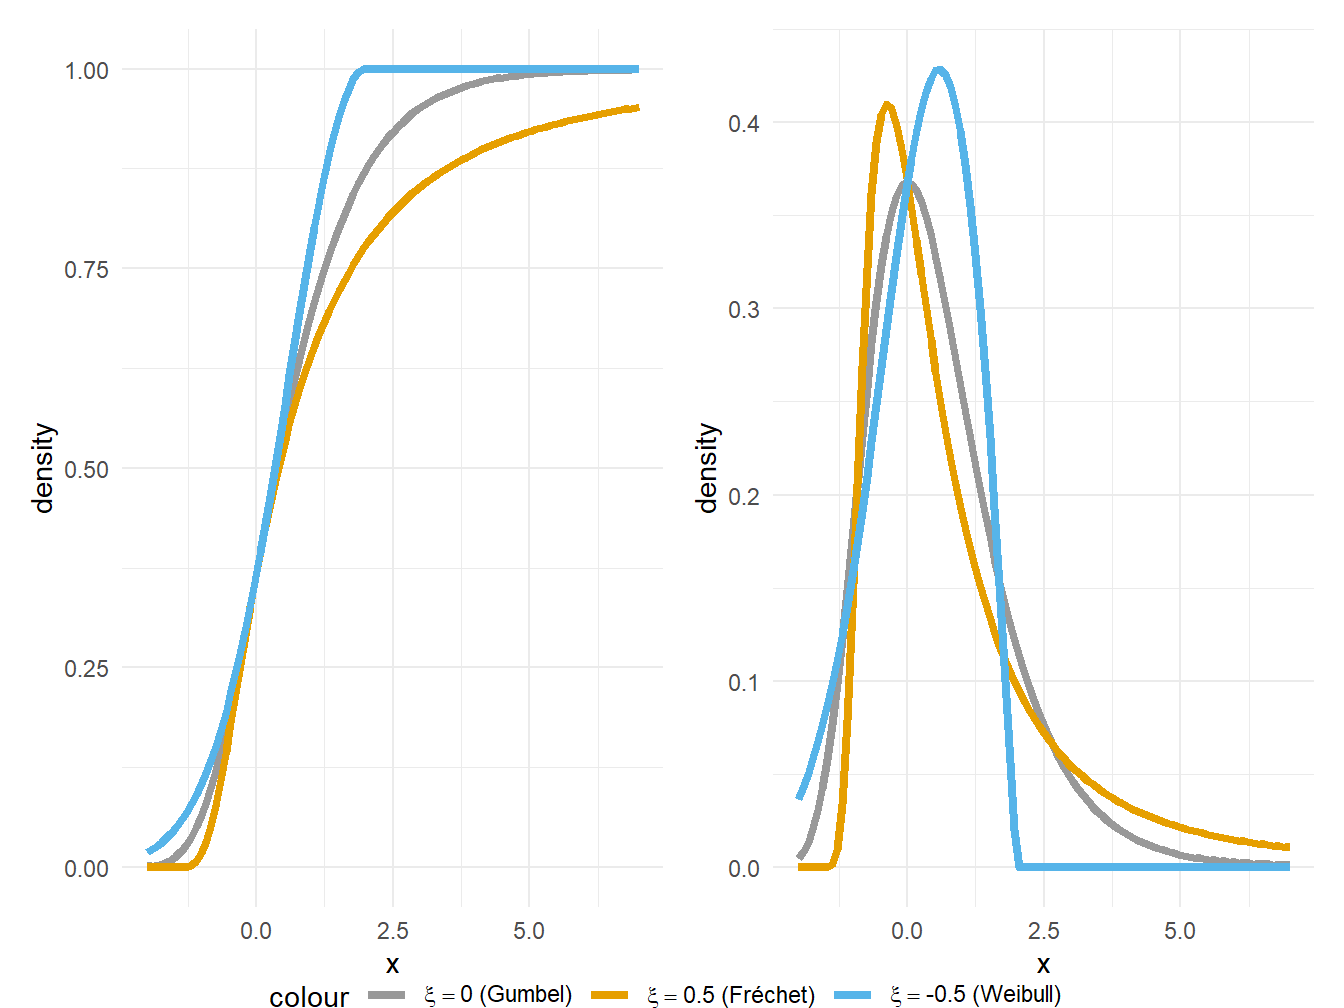
\includegraphics[width=1\linewidth]{thesis_files/figure-latex/gevDist-1} 

}

\caption{The df (left) and density (right) of a standard GEV distribution in three cases, corresponding to the Gumbel, Fréchet and Weibull distributions, respectively.}\label{fig:gevDist}
\end{figure}
Now, supposing that the maxima \(M_n\) of independently and identically distributed random variables converge in distribution as \(n \rightarrow \infty\) under an appropriate normalization. Having that \(P(M_n \leq x) = F^{n}(x)\), this convergence means that there exists sequences of real constants \(d_n\) and \(c_n\) where \(c_n > 0\) for all \(n\) such that
\begin{equation}
\lim_{n \to \infty} P((M_n - d_n)/c_n \leq x) = \lim_{n \to \infty} F^{n}(c_{n}x + d_n) = H(x),
\label{eq:limitingdist}
\end{equation}
for some non-degenerate distribution function \(H(x)\). The role of the GEV distribution in the study of maxima is formalized by the following definition and theorem.
\begin{definition}[Maximum domain of attraction]
\protect\hypertarget{def:unnamed-chunk-1}{}{\label{def:unnamed-chunk-1} \iffalse (Maximum domain of attraction) \fi{} }
If Equation \eqref{eq:limitingdist} holds for some non-degenerate distribution function \(H\), then \(F\) is said to be in the maximum domain of attraction (MDA) of \(H\), written \(F \in \text{MDA}(H)\).
\end{definition}
\begin{theorem}[The Fisher-Tippett-Gnedenko theorem]
\protect\hypertarget{thm:gnedenko}{}{\label{thm:gnedenko} \iffalse (The Fisher-Tippett-Gnedenko theorem) \fi{} }
If \(F \in \text{MDA}(H)\) for some non-degenerate distribution function \(H\), then \(H\) must be a distribution of type \(H_{\xi}\), i.e.~a GEV distribution.
\end{theorem}
\hypertarget{peaks-over-threshold-based-models}{%
\subsubsection{Peaks-over-threshold-based models}\label{peaks-over-threshold-based-models}}

As was mentioned in the introduction to this section, the BM method has the major defect of being very wasteful of valuable data since it only retains the maximum losses in large blocks. In contrast, methods based on so-called threshold exceedances or \emph{peaks-over-thresholds} uses all data that exceed a particular threshold. The main distribution model for such exceedances over thresholds is the generalized Pareto distribution (GPD), which is introduced next.

For a random quantity \(X\) with distribution function \(F(x)\), Pickands (1975) has shown that under certain conditions, \(F(x \vert u) = P(X \leq u +x\vert X>u)\) can be approximated by a GPD, which is defined as follows.
\begin{definition}[GPD]
\protect\hypertarget{def:gpd}{}{\label{def:gpd} \iffalse (GPD) \fi{} }
The distribution function of the GPD is given by
\begin{equation}
G_{\xi, \beta}(x) = 
\begin{cases}
1 - (1 + \xi x / \beta)^{-1/\xi}, & \text{if}\ \xi \ \neq\ 0 \\
1 - \exp(-x\beta), & \text{if}\ \xi \ =\ 0, 
\end{cases}
\label{eq:GPD}
\end{equation}
\end{definition}
Like the GEV distribution defined in Definition \ref{def:gev}, the GPD is generalized in the sense that it contains a number of special cases: when \(\xi > 0\) the distribution function \(G_{\xi, \beta}\) is that of an ordinary Pareto distribution with \(\alpha = 1/\xi\). When \(\xi = 0\), we have an exponential distribution and when \(\xi < 0\) we have a short-tailed Pareto type II distribution. Figure \ref{fig:gpdDist} shows the GPD distribution function and density for these three different cases.
\begin{figure}[H]

{\centering 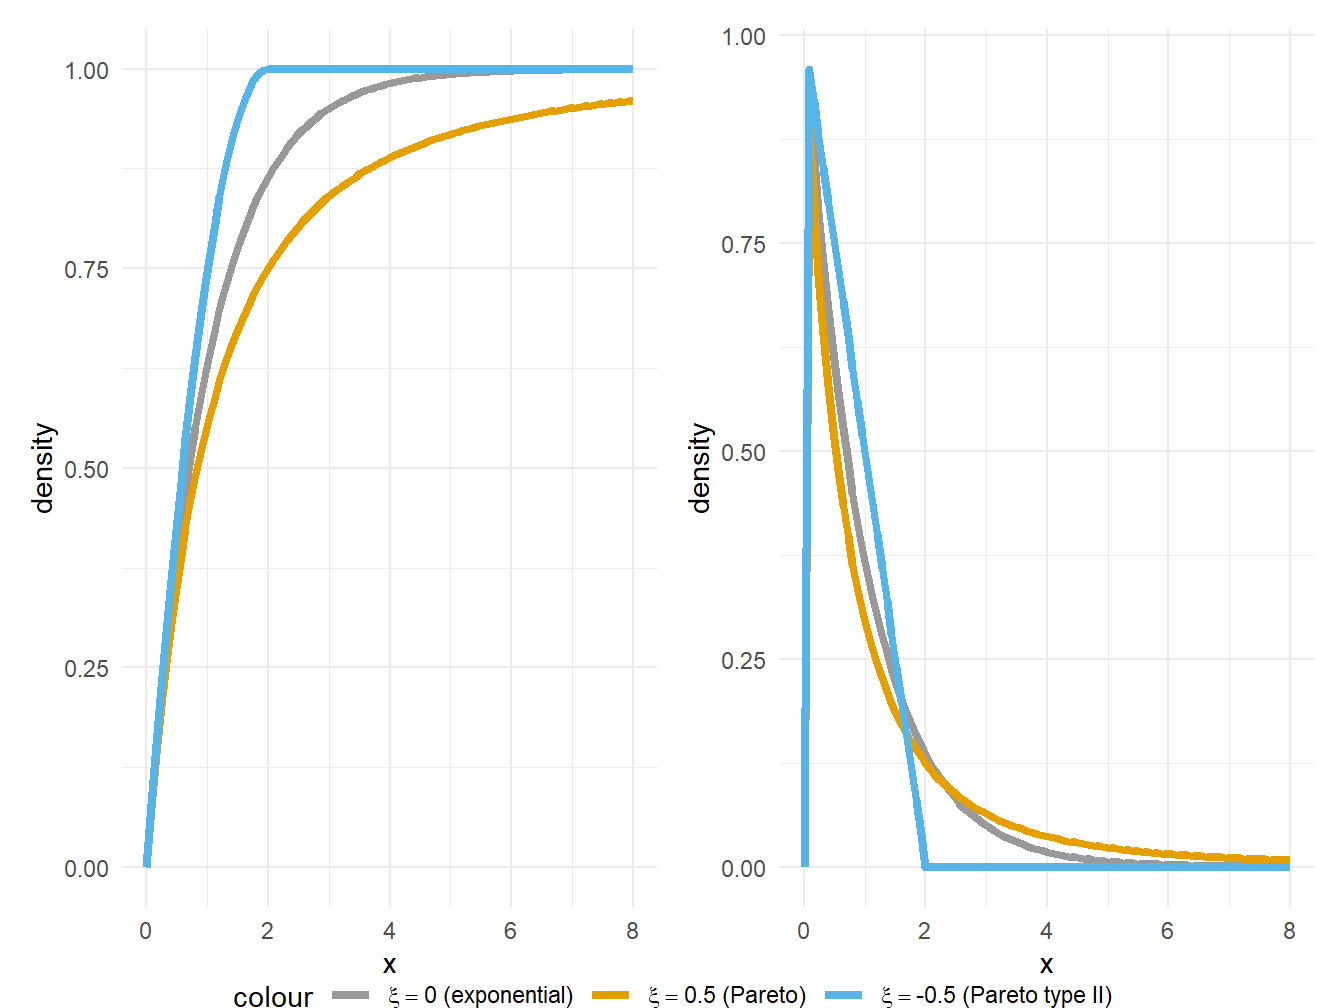
\includegraphics[width=1\linewidth]{thesis_files/figure-latex/gpdDist-1} 

}

\caption{The df (left) and density (right) of a standard GPD distribution in three cases, corresponding to the exponential, Pareto and Pareto type II distributions, respectively.}\label{fig:gpdDist}
\end{figure}
The role of the GPD in EVT is as a natural model for the so-called \emph{excess distribution} over a high threshold, which is defined as follows.
\begin{definition}[Excess distribution over threshold $u$]
\protect\hypertarget{def:excessdist}{}{\label{def:excessdist} \iffalse (Excess distribution over threshold \(u\)) \fi{} }
Let \(X\) be a random variable with distribution function \(F\). The excess distribution over the threshold \(u\) has distribution function
\begin{equation}
F_{u}(x) = P(X - u \leq x \vert X > u) = \frac{F(x + u) - F(u)}{1 - F(u)},
\label{eq:excessdist}
\end{equation}
for \(0 \leq x < x_F - u\), where \(x_F \leq \infty\) is the right endpoint of \(F\).
\end{definition}
A related concept that also plays an important role in EVT is that of the \emph{mean excess function}, which has the following definition.
\begin{definition}[Mean excess function]
\protect\hypertarget{def:meanexcess}{}{\label{def:meanexcess} \iffalse (Mean excess function) \fi{} }
The mean excess function of a random variable \(X\) with finite mean is given by
\begin{equation}
e(u) = E(X - u \vert X > u).
\label{eq:meanexcess}
\end{equation}
\end{definition}
The excess distribution function \(F_u\) describes the distribution of the excess loss over the threshold \(u\), given that \(u\) is exceeded. The mean excess function \(e(u)\) expresses the mean of \(F_u\) as a function of \(u\). In general, if X has distribution function \(F = G_{\xi, \beta}\), then, following Equation \eqref{eq:excessdist}, the excess distribution function is
\begin{equation}
F_{u}(x) = G_{\xi, \beta (u)}(x), \quad \beta (u) = \beta + \xi u,
\label{eq:excessdistGPD}
\end{equation}
where \(0 \leq x < \infty\) if \(\xi \geq 0\) and \(0 \leq x \leq -(\beta / \xi) - u\) if \(\xi < 0\). Using Equation \eqref{eq:excessdistGPD} and the mean of the GPD, which is \(E(X) = \beta / (1-\xi)\), the mean excess function of the GPD can be found to equal
\begin{equation}
e(u) = \frac{\beta (u)}{1 - \xi} = \frac{\beta + \xi u}{1 - \xi},
\label{eq:meanexcessGPD}
\end{equation}
where \(0 \leq u < \infty\) if \(0 \leq \xi < 1\) and \(0 \leq u \leq -\beta / \xi\) if \(\xi < 0\). The mean excess function is linear in the threshold \(u\), which is one of the characterizing properties of the GPD.

The following theorem shows that the GPD is a natural limiting excess distribution for many underlying loss distributions.
\begin{theorem}[The Pickands-Balkema-de Haan theorem]
\protect\hypertarget{thm:pickands}{}{\label{thm:pickands} \iffalse (The Pickands-Balkema-de Haan theorem) \fi{} }
We can find a (positive-measurable function) \(\beta (u)\) such that
\begin{equation}
\lim_{u \to x_F} \sup_{0 \leq x < x_{F-u}} \vert F_{u}(x) - G_{\xi, \beta (u)} (x) \vert = 0,
\label{eq:pickands}
\end{equation}
if and only if \(F \in \text{MDA} (H_{\xi}), \xi \in \mathbb R\)
\end{theorem}
Theorem \ref{thm:pickands} is a very widely applicable result that essentially shows that the GPD is the \emph{canonical distribution} for modeling excess losses over high thresholds. It underlies modeling based on the GPD.

Figure \ref{fig:bmpotplot} gives a graphical representation of the conceptual difference between the BM model (left panel) and the POT model (right panel). As seen, the BM model considers the maximum value for a specific time period, e.g.~monthly or yearly, where the variables \(X_2, X_5, X_7\) and \(X_{11}\) correspond to the block maxima for each such period. The POT model instead considers all observations above a specified threshold (represented by the gray horizontal line), in which case the variables \(X_1, X_2, X_5, X_7, X_8, X_9\) and \(X_{11}\) are considered as the extreme events.
\begin{figure}[H]

{\centering \includegraphics[width=0.8\linewidth]{thesis_files/figure-latex/bmpotplot-1} 

}

\caption{A graphical representation of the difference between the BM model (left) and the POT model (right).}\label{fig:bmpotplot}
\end{figure}
\hypertarget{sec:modelingrisk}{%
\subsubsection{Modeling risk measures with EVT}\label{sec:modelingrisk}}

\hypertarget{modeling-excess-losses}{%
\paragraph{Modeling excess losses}\label{modeling-excess-losses}}

As has been stated in the above, the focus of this thesis will be on POT models. POT models use the GPD as the main distribution model for exceedances over thresholds.

We first circle back to Theorem \ref{thm:pickands}. Assuming that we have a loss distribution \(F \in \text{MDA}(H_\xi)\) such that, for some high threshold \(u\), we can model \(F_u\) by a GPD. This builds on the assumption that \(F\) is a loss distribution with right endpoint \(x_F\) and that we for some high threshold \(u\) have \(F_{u}(x)=G_{\xi, \beta}(x)\) for \(0 \leq x < x_F-u\) and some \(\xi \in \mathbb R\) and \(\beta > 0\).

The method for modeling exceedances is then as follows. Given loss data \(X_1, X_2, \dots, X_n\) from \(F\), a random number of observations will exceed the threshold \(u\). Labeling the total number of observations exceeding the threshold \(u\), i.e.~the total number of exceedances, as \(N_u\) and the corresponding observations as \(\tilde X_1, \tilde X_2, \dots, \tilde X_n\), we calculate \(Y_j = \tilde X_j - u\) of the excess loss for each of these exceedances. The aim is to estimate the parameters of a GPD model by fitting the distribution to the \(N_u\) excess losses. This can be done in several ways, with the most common method being by way of maximum likelihood estimation, a method which has been extensively studied in an EVT framework (examples include Davison (1984), Smith (1984) and Grimshaw (1993)). Alternative methods include the probability-weighted moment (PWM) method (Hosking and Wallis, 1987) and the elemental percentile method (Castillo and Hadi, 1997). In this thesis, the focus will be on maximum likelihood estimation. The method of finding the maximum likelihood estimates of the GPD is shown in Appendix \ref{sec:mle}.

\hypertarget{choice-of-threshold}{%
\paragraph{Choice of threshold}\label{choice-of-threshold}}

Utilising the POT method to model extreme values requires that a suitable threshold \(u\) is chosen. This threshold basically serves as a cut-off above which the GPD is (hopefully) a suitable model. The choice of the threshold \(u\) is for this reason an important, but unfortunately not a trivial, task. The higher the threshold is set, the fewer observations there are for estimating the parameters of the GPD, making the estimates less reliable. A lower threshold implies that more observations are available for parameter estimation, but comes with the trade-off that observations above the (lower) threshold might not conform to the GPD (Christoffersen, 2011). There exists no readily applicable algorithm (yet) for selecting a suitable threshold (Gilli and Këllesi, 2006). One common method for trying to make an informed decision regarding the choice of threshold builds on the \emph{mean excess function}, which is given by
\begin{equation}
e(v) = \frac{\beta + \xi (v-u)}{1-\xi} = \frac{\xi v}{1 - \xi} + \frac{\beta - \xi u}{1 - \xi},
\label{eq:meanexcessfunction}
\end{equation}
where \(u \leq v < \infty\) if \(0 \leq \xi < 1\) and \(u \leq v \leq u - \beta/\xi\) if \(\xi < 0\). The mean excess function in Equation \eqref{eq:meanexcessfunction} is linear in \(v\), and this is commonly exploited as the basis for a graphical method for choosing an appropriate threshold based on the so-called \emph{sample mean excess plot}.

For positive-valued loss data \(X_1, X_2, \dots, X_n\), the sample mean excess function is defined to be an empirical estimator of the mean excess function in Definition \ref{def:meanexcess}, the estimator of which is given by
\begin{equation}
e_{n}(v) = \frac{\sum_{i=1}^{n}(X_i - v)I_{\{X_i > v\}}}{\sum_{i =1}^{n}I_{\{X_i > v\}}}.
\label{eq:meanexcessest}
\end{equation}
A mean excess plot is then constructed. If the data support a GPD model over a high threshold, then Equation \eqref{eq:meanexcessfunction} suggests that this plot should become increasingly ``linear'' for higher values of \(v\). In this context, a linear upward trend indicates a GPD model with positive shape parameter \(\xi\) and a plot tending towards being horizontal indicates a GPD with approximately a zero shape parameter, i.e.~an exponential excess distribution. Finally, a linear downward trend indicates a GPD with a negative shape parameter.

An example\footnote{The data comes from the well-studied Danish fire insurance data, which consists of 2,156 fire insurance losses over 1,000,000 Danish kroner from 1980 to 1990, expressed in units of 1,000,000 kroner. Data accessed via the function \texttt{data(danish)} in the \texttt{\{evir\}} R package.} of a sample mean excess plot is shown in Figure \ref{fig:meplotex}.
\begin{figure}[H]

{\centering \includegraphics[width=0.8\linewidth]{thesis_files/figure-latex/meplotex-1} 

}

\caption{Example of a sample mean excess plot based on the Danish fire insurance dataset.}\label{fig:meplotex}
\end{figure}
Here, we see that the plot is fairly linear over the entire range, and the upwards slope suggests that a GPD with a positive shape parameter \(\xi\) could be fitted for the data. There is a small kink forming after a threshold of 10, which suggests that \(u = 10\) might be a sensible starting point as a choice of threshold.

The method of using the sample mean excess plot for determining a suitable threshold suffers from the major drawback of being subjective (and sometimes highly so); it is not always apparent when and where the linearity ``ceases'' and there can also be several distinct linear parts. As an alternative, the threshold can simply be set such that some proportion of the distribution is above the threshold. Nyström and Skoglund (2002) suggests that the threshold be set such that 10\% of the distribution is above the threshold; other choices that could be equally suitable are 5\% and 15\%.

\hypertarget{estimation-of-the-tail-and-risk-measures}{%
\paragraph{Estimation of the tail and risk measures}\label{estimation-of-the-tail-and-risk-measures}}

Using the GPD model described previously to model excess losses, we can proceed to estimate the tail of the underlying loss distribution \(F\) and the associated risk measure, in this case ES.

The formula for \emph{tail probabilities}, for \(x \geq u\), is given by
\begin{equation}
\begin{aligned}
\bar F (x) &= P(X >u)P(X > x \vert X >u)\ \\
& = \bar F (u)P(X-u > x- u \vert X > u)\ \\
& = \bar F (u) \bar F_u (x-u)\ \\
& = \bar F (u) \left(1 + \xi \frac{x-u}{\beta} \right)^{-1\xi}.
\end{aligned}
\label{eq:tailprob}
\end{equation}
By inverting Equation \eqref{eq:tailprob}, we can obtain a high quantile of the underlying distribution, which in turn can be interpreted as VaR. Then, for \(\alpha \geq F(u)\), VaR equals
\begin{equation}
\text{VaR}_{\alpha} = q_{\alpha}(F) = u + \frac{\beta}{\xi} \left( \left (  \frac{1-\alpha}{\bar F(u)}  \right)^{-\xi} -1 \right).
\label{eq:VaRest}
\end{equation}
For \(\xi < 1\), the ES is calculated as
\begin{equation}
\text{ES}_{\alpha} = \frac{1}{1-\alpha} \int_{\alpha}^{1} q_{x}(F)\text{dx} = \frac{\text{VaR}_{\alpha}}{1 - \xi} + \frac{\beta - \xi u}{1 - \xi}.
\label{eq:ESest}
\end{equation}
If a GPD has been fitted to excess losses over a threshold \(u\) in the manner described above, the quantities can be estimated by replacing \(\xi\) and \(\beta\) in Equations \eqref{eq:tailprob}--\eqref{eq:ESest} by their corresponding estimates. This also requires an estimate of \(\bar F(u)\), for which the simple empirical estimator \(N_u/n\) is often used.\footnote{By using the empirical estimator \(N_u/n\), we are implicitly assuming that there is a sufficient proportion of sample values above the threshold \(u\) to reliably estimate \(\bar F(u)\).} An estimator for tail probabilities, which was first proposed by Smith (1987), can then be obtained, on the form
\begin{equation}
\hat{\bar{{F}}}(x) = \frac{N_u}{n}\left(1 + \hat \xi \frac{x - u}{\hat \beta} \right)^{-1/ \hat \xi}.
\label{eq:tailprobest}
\end{equation}
Equation \eqref{eq:tailprobest} is, however, only valid for \(x \geq u\).

For \(\alpha \geq 1 - N_u\), analogous point estimators of \(\text{VaR}_{\alpha}\) and \(\text{ES}_{\alpha}\) are obtained from Equations \eqref{eq:VaRest} and \eqref{eq:ESest}. To do this, we can set a high threshold \(u = L_{k+1, n}\) at the \((k+1)\)-upper-order statistic and fit a GPD distribution to excess losses over \(u\). It is thereby possible to obtain the maximum likelihood estimates \(\hat \xi\) and \(\hat \beta\) based on \(k\) exceedances over the threshold. In order to form a quantile estimator, the value \(k\) must satisfy \(k/n > 1 - \alpha\), where \(k\) should be sufficiently large to give reasonably accurate estimates of the GPD parameters. It follows then that the risk measure estimates for \(\text{VaR}_{\alpha}\) and \(\text{ES}_{\alpha}\), respectively, are
\begin{equation}
\widehat{\text{VaR}}_{\alpha} = u + \frac{\hat \beta}{\hat \xi}\left(\left( \frac{1-\alpha}{k/n} \right)^{- \hat \xi} -1 \right),
\label{eq:VaRestimate}
\end{equation}
\begin{equation}
\widehat{\text{ES}}_{\alpha} = \frac{\widehat{\text{VaR}}_{\alpha}}{1-\hat \xi} + \frac{\hat \beta - \hat \xi u}{1-\hat \xi}.
\label{eq:ESestimate}
\end{equation}
\hypertarget{sec:data}{%
\section{Data and methodology}\label{sec:data}}

\hypertarget{methodological-aspects}{%
\subsection{Methodological aspects}\label{methodological-aspects}}

\hypertarget{financial-returns}{%
\subsubsection{Financial returns}\label{financial-returns}}

Our main interest in the context of this thesis are the \emph{returns} of financial assets. More specifically, we are interested in the (large) negative returns, more commonly known as losses. If we let \(P_t\) represent the daily closing price of a particular assets at time \(t\), the simple gross return \(R_t\), i.e.~the return from \(t-1\) to \(t\), is defined as
\begin{equation}
1 + R_t = \frac{P_t}{P_{t-1}}.
\label{eq:grossreturn}
\end{equation}
The continuously compounded return (the ``log return''), \(r_t\), is then defined as the natural logarithm of Equation \eqref{eq:grossreturn}, that is
\begin{equation}
r_t = \text{log}(1 + R_t) = \text{log}(\frac{P_t}{P_{t-1}}) = \text{log}(P_t) - \text{log}(P_{t-1}).
\label{eq:logreturn}
\end{equation}
The so-called loss return \(X_t\) at time \(t\) represents the negative log-return \(r_t\) and is thus defined simply as
\begin{equation}
X_t = -r_t.
\label{eq:lossreturn}
\end{equation}
\(X_t\) therefore represents losses as positive values. The percentage \emph{loss} in value from time \(t-1\) to \(t\) is then calculated as
\begin{equation}
L_t = 100(1-\text{exp}(r_t)) = 100(1-\text{exp}(-X_t)),
\label{eq:percloss}
\end{equation}
where positive values of \(L_t\) represent percentage losses and negative values represent percentage gains. Since we are interested in the large losses in the context of this thesis, the general focus will be on daily values of \(L_t > 0\), which, as said, represents the daily percentage losses.

\hypertarget{implementation}{%
\subsubsection{Implementation}\label{implementation}}

The implementation of the theoretical aspects and their application to the empirical data is done via R (R Core Team, 2013). EVT-specific applications have been made available through the R packages \texttt{\{evir\}} (Pfaff and McNeil, 2018) and \texttt{\{qrmtools\}} (Hofert, Hornik and McNeil, 2021), which have been used for these purposes in this thesis.

\hypertarget{data-exposition}{%
\subsection{Data exposition}\label{data-exposition}}

As was stated in the introduction, the estimation ES will be performed on data representing (or trying to represent) the entire spectrum of the financial markets, namely equity, fixed income, currency exchange rates, commodities, and, in the name of modernity, cryptocurrencies. Equity will be represented by the Swedish OMXS30 index\footnote{The OMXS30 price data comes from www.borsdata.se (paid subscription).}, which represents the 30 largest companies on the Nasdaq Stockholm exchange. Fixed income is represented by the OMRXBOND index\footnote{The OMRXBOND price data comes from www.nasdaqomxnordic.com.}, which includes bonds issued by the Swedish state. Currency exchange rates will be represented by the SEK/EUR exchange rate and commodities gets its representation through Brent crude\footnote{The SEK/EUR and Brent crude price data comes from www.borsdata.se (paid subscription).}, which also serves a function as a reference for pricing oil, making it suitable as a broad representation of commodities. Lastly, cryptocurrencies is represented by what most think of when it comes to this asset class -- the ``millennials' gold'' -- namely, Bitcoin\footnote{The Bitcoin price data comes from www.coindesk.com.}.

The data consists of daily closing prices for each of the assets. For each observation, the log return was first computed (which excludes the first observation in each series) as per Equation \eqref{eq:logreturn}. From this, the daily percentage losses were calculated as per Equation \eqref{eq:percloss}. Table \ref{tab:descriptives} gives an overview of the start date, end date and number of observations for the data pertaining to each asset class.
\begin{table}[H]

\caption{\label{tab:descriptives}Start and end date of each time series and the number of observations.}
\centering
\begin{tabular}[t]{cccc}
\toprule
\textbf{Asset} & \textbf{Start} & \textbf{End} & \textbf{N}\\
\midrule
OMXS30 & 2001-04-23 & 2021-04-20 & 5014\\
Bitcoin & 2011-08-18 & 2021-04-18 & 3466\\
Brent crude & 2001-04-23 & 2021-04-19 & 5116\\
SEK/EUR & 2001-04-23 & 2021-04-19 & 4610\\
OMRXBOND & 2005-04-19 & 2021-04-22 & 4009\\
\bottomrule
\end{tabular}
\end{table}
Figure \ref{fig:assets} shows the daily closing price and the (positive and negative) percentage losses for each asset class for the relevant period.
\begin{figure}[H]

{\centering \includegraphics[width=1\linewidth]{thesis_files/figure-latex/assets-1} 

}

\caption{Daily closing prices (left) and percentage losses (right) of each asset.}\label{fig:assets}
\end{figure}
From Figure \ref{fig:assets}, we can see clear signs of the phenomenon known as \emph{volatility clustering}, i.e.~that large changes tend to be followed by large changes and small changes tend to be followed by small changes (though not necessarily in the same direction).\footnote{Volatility clustering was first observed by Mandelbrot (1963) and the empirical property has been document by Granger and Ding (1995) and Ding and Granger (1996), among many others.}

Table \ref{tab:table1} gives an overview of the descriptive statistics for the percentage loss data for the assets.
\begin{table}[H]

\caption{\label{tab:table1}Descriptives statistics for each asset.}
\centering
\begin{tabular}[t]{ccccccc}
\toprule
\textbf{Asset} & \textbf{Mean} & \textbf{Std.Dev.} & \textbf{Skewness} & \textbf{Kurtosis} & \textbf{Min} & \textbf{Max}\\
\midrule
OMXS30 & 0.00862 & 1.41419 & -0.23673 & 8.08447 & -11.82074 & 9.39406\\
Bitcoin & 0.11926 & 5.24591 & -3.67845 & 58.09043 & -94.24460 & 35.95238\\
Brent crude & -0.00862 & 2.32730 & -1.13750 & 20.62332 & -32.28143 & 17.36807\\
SEK/EUR & -0.00321 & 0.46580 & -0.19918 & 6.70325 & -3.13448 & 3.25843\\
OMRXBOND & 0.01126 & 0.12122 & 0.16445 & 7.03015 & -0.86665 & 0.88648\\
\bottomrule
\end{tabular}
\end{table}
There are some things to note in Table \ref{tab:table1}. First, we can see that Bitcoin had both the largest daily gain and largest daily loss during the relevant period, with the largest daily gain being substantially higher than the largest daily loss. Second place in this category is taken by Brent crude, which also exhibit rather large daily swings during the period. The SEK/EUR currency and the OMRXBOND index proved to be the least volatile in terms of daily swings during the period, with the OMXS30 being somewhere in the middle.

Of particular note here is the kurtosis. Kurtosis is a measure of the ``tailedness''\footnote{Kurtosis is a measure of ``tailedness'', i.e.~how the tails of a probability distribution behaves and is defined as \(\text{Kurt}[X] = \frac{E[(X-\mu)^4]}{(E[(X-\mu)^2])^2}\). The more the kurtosis differs from 3, the ``fatter'' the tails of the distribution. There is a common misconception that kurtosis also measures the ``peakedness'' of a distribution, but this notion is dispelled by Westfall (2014).} of a distribution. The normal distribution has a kurtosis of 3, and a distribution with a kurtosis deviating from this value suggests fatter tails and thus, that a normality assumption might not be an appropriate approximation for the underlying distribution. From the above, we see that all assets have a kurtosis above 3, which therefore suggests that they are heavy-tailed (or at least ``heavier-tailed'' than the normal distribution). To the surprise of no one, Bitcoin and Brent crude exhibits the highest kurtosis of the assets.

Lingering on the kurtosis point, we can further investigate the kurtosis by examining so-called quantile-quantile (Q-Q) plots, shown in Figure \ref{fig:qqplots}.
\begin{figure}[H]

{\centering \includegraphics[width=1\linewidth]{thesis_files/figure-latex/qqplots-1} 

}

\caption{Q-Q plots for each asset, comparing sample quantiles to the theoretical quantiles.}\label{fig:qqplots}
\end{figure}
If the data came from a normal distribution, the sample points would line on a straight line with the theoretical quantiles. From the above, we see quite clearly that a normality assumption is not realistic for these series since the tails are heavier, confirming what we saw in terms of kurtosis. This does indeed suggest that an EVT approach is reasonable for estimating ES on the basis of these time series, which we turn to next.

\newpage

\hypertarget{sec:results}{%
\section{Results}\label{sec:results}}

\hypertarget{estimating-the-excess-losses}{%
\subsection{Estimating the excess losses}\label{estimating-the-excess-losses}}

The first step in estimating ES is to model the excess losses for each of the assets, which in this thesis is done according to the unconditional POT model as further described in Section \ref{sec:method} above.

Modeling the excess losses first requires choosing an adequate threshold \(u\) above which we fit a GPD to the excess losses, hoping to obtain an adequate model for the largest -- the most extreme -- losses. The choice of the threshold \(u\) will in this thesis be made through the inspection of mean excess plots, following the methodology outlined in Section \ref{sec:modelingrisk}. Even though this method is somewhat (and sometimes highly) subjective, as mentioned earlier, it is one of the few methods available for the purpose of making an informed decision about a suitable threshold. Figures \ref{fig:omxs30meplot}--\ref{fig:treasurymeplot} in Appendix \ref{sec:meplots} shows the mean excess plots of the \emph{positive} daily percentage losses \(L_t\) for each asset, i.e.~negative percentage losses (gains) are omitted in these plots (since they do not interest us in this context).

As can be seen in these mean excess plots, none of them are perfectly linear (or even close to being perfectly linear). This obviously makes the choice of threshold more difficult, since what we are looking for is a point in the plot after which there is a somewhat stable linearity present, with the absence of any wild swings up or down. However, even for data that are truly generalized Pareto distributed, the sample mean excess plot is seldom perfectly linear, which is especially apparent towards the right-hand end of the plot. This is so because we are here averaging a small number of excesses (since the very extreme values are few). These end-points are often omitted from consideration as they can distort the overall picture. McNeil, Frey and Embrechts (2015) suggest that, if there is visual evidence that the mean excess plot shows a trend of (stable) linearity, the threshold \(u\) should be set to a value towards the beginning of the linear section of the mean excess plot.

Following this recommendation, the threshold for each asset is chosen at a point where the mean excess plot gives a visual indication of a budding and stable linearity. This, as pointed out above, is indeed a highly subjective exercise. The threshold values chosen have been marked with a vertical line in the respective mean excess plot, and their exact numerical values are shown in Table \ref{tab:pointestimates}.

With a method this subjective, the last thing we want is for the chosen threshold to have a large impact on the subsequent estimation procedure, especially the shape parameter \(\xi\). One way to further guide the decision of a suitable threshold is to fit the GPD shape parameter \(\xi\) as a function of the threshold and plot these for a range of threshold values. Such plots are called \emph{shape plots}. Using shape plots, we are then able to visualize how the shape parameter \(\xi\) is affected by different values of \(u\). Shape plots for each of the assets are shown in Appendix \ref{sec:shapeplots}. The Y-axis of these plots shows different values of the shape parameter \(\xi\) (solid line), together with 95\% confidence bands (dotted lines). The lower X-axis shows the value of the threshold and the upper X-axis the number of excesses (which decreases with an increasing threshold value \(u\)). The vertical line represents the threshold \(u\) chosen previously and the horizontal line represents a value of the shape parameter \(\xi = 0.25\), above which line the models have an infinite fourth moment (kurtosis), i.e.~the tail ``never ends''. Obviously, we want the value of \(\xi\) to be stable for as large a range of threshold values as possible, i.e.~the line should be as flat as possible after the point of the threshold.

For the OMXS30 percentage loss data, the threshold chosen after inspection of the mean excess plot was \(u =\) 1\%. We see in Figure \ref{fig:omxs30shapeplot} that the value of the shape parameter \(\xi\) remains fairly stable up to a value of \(u\) of about 3, after which point it starts a somewhat linear increase. The mean excess plot does indeed suggest that a threshold can be found above which a GPD approximation to the excess distribution is reasonable. The value of the threshold \(u\) chosen initially for these data seems to be reasonable as it is within the range mentioned previously, i.e.~where there is a flat trend in the relevant shape plot.

As seen in Figure \ref{fig:bitcoinshapeplot}, the threshold for the Bitcoin percentage loss data was chosen at the very start of the series, and we see in the shape plot that the shape parameter \(\xi\) remains remarkably stable throughout a range of threshold values, and never crosses the horizontal line. Again, it should be possible to fit a GPD to the excesses above the threshold and achieve a sensible model. Thus, the conclusion here is that the threshold chosen for Bitcoin percentage loss data, \(u =\) 0.25\%, seems to be reasonable, and it will be the value used in the subsequent estimation.

Figure \ref{fig:brentshapeplot} shows the shape plot for the Brent crude percentage loss data. We see that the value of the shape parameter \(\xi\) remains fairly stable in the approximate range of \(2\)\% \(< u <\) \(3\)\%, after which there is an initial increase and a subsequent (linear) decrease. The threshold chosen for the Brent crude data based on the corresponding mean excess plot is \(u =\) 2.3\%, which seems reasonable here since it is within the ``stable range'' indicated above. The conclusion is that it also for the Brent crude percentage loss data should be possible to fit a GPD to approximate the excess distribution.

For the SEK/EUR percentage loss data, we see in Figure \ref{fig:sekshapeplot} that the shape parameter \(\xi\) is highly unstable, with no signs of a flat trend. The threshold chosen, \(u =\) 0.82\%, is slightly above the point at which the model has infinite kurtosis. Here, the choice of threshold is difficult since, as said, there is no clear flat trend apparent in the plot. For now, the threshold chosen initially will be kept. At this stage however, it is unclear whether the GPD is suitable for modeling the excess distribution, a point which we will have reasons to return to.

Finally, the OMRXBOND percentage loss data in Figure \ref{fig:treasuryshapeplot} shows that the threshold \(u =\) 0.25\% intersects at a point at which the shape plot line starts to flatten out and show a somewhat stable trend, but only until a threshold of around \(u = 0.28\)\% is reached, after which there is some up-and-down gyration. The initial threshold chosen does seem reasonable, at least for a narrow range of threshold values. Based on this information, it is reasonable to assume that a GPD can be fitted to the excess distribution (this point will also be returned to later).

One additional thing to note in the shape plots for all assets is that the confidence intervals widens with an increasing threshold; this further stresses the importance of choosing a threshold that is not too high as the parameter estimates -- the shape parameter \(\xi\) in this case -- becomes increasingly uncertain.

With the thresholds thus chosen, we are able to calculate the excesses above the threshold for the respective asset. To determine whether a GPD approximation to the excess distribution \(\hat F(x-u)\) is reasonable for each asset, Figures \ref{fig:empomxs30}--\ref{fig:emptreasury} in Appendix \ref{sec:empplots} shows plots of the empirical distribution of excesses and the fitted GPD. For these, we see a very good correspondence between the empirical estimates and the GPD curve for the OMXS30, Bitcoin and Brent crude percentage loss data. The difficulties posed by the SEK/EUR data in choosing a threshold is confirmed by the corresponding empirical distribution plot; the correspondence between the empirical estimates and the GPD curve is less than satisfactory, implying that a GPD might not be a suitable approximation for this data. The OMRXBOND percentage loss data gives a somewhat similar picture, indicating that a GPD may be an unsuitable model for that data as well.

Table \ref{tab:pointestimates} gives an overview of the threshold \(u\), the number of exceedances \(N_u\) (with the proportion of the total observations above the threshold within parentheses) as well as point estimates for the shape parameter \(\xi\) and the scale parameter \(\beta\) (with the standard error for the respective parameter estimate within parentheses) for each asset.
\begin{table}[H]

\caption{\label{tab:pointestimates}Overview of the threshold, the number of exceedances and point estimates of the shape and scale parameter for each of the assets.}
\centering
\begin{tabular}[t]{ccccc}
\toprule
\textbf{Asset} & \textbf{$u$} & \textbf{$N_u$} & \textbf{$\hat \xi$} & \textbf{$\hat \beta$}\\
\midrule
OMXS30 & 1.00 & 907 (0.181) & 0.127 (0.038) & 0.799 (0.040)\\
Bitcoin & 0.25 & 1722 (0.497) & 0.156 (0.029) & 2.396 (0.089)\\
Brent crude & 2.30 & 555 (0.108) & 0.144 (0.048) & 1.270 (0.081)\\
SEK/EUR & 0.82 & 159 (0.034) & 0.223 (0.112) & 0.243 (0.033)\\
OMRXBOND & 0.25 & 105 (0.026) & 0.246 (0.130) & 0.076 (0.012)\\
\bottomrule
\end{tabular}
\end{table}
There are a few observations to be made in relation to Table \ref{tab:pointestimates}. First of all, we see that almost half of all observations for the Bitcoin percentage loss data is above the threshold chosen for the data. This proportion is much higher than for even the data with the second highest proportion of observations above the threshold, being the OMXS30 percentage loss data. We can also note that a very small proportion of the total observations are above the chosen threshold for the SEK/EUR and the OMRXBOND percentage loss data. The proportion of observations above the threshold is obviously directly determined by the threshold chosen for the data (which in this thesis was made on the basis of mean excess plots). It is, however, interesting to see the large differences between the assets in this respect.

As regards the standard errors for the estimates of the shape parameter \(\xi\) and the scale parameter \(\beta\), we see that these are fairly small for the OMXS30, Bitcoin and Brent crude percentage loss data. The standard errors for the SEK/EUR and OMRXBOND percentage loss data, however, are high, at least in relation to the standard errors for the other assets just mentioned. These larger standard errors for the SEK/EUR and OMRXBOND percentage loss data are no doubt (at least partially) a consequence of the small proportion of observations above the threshold. This is the case since the fewer observations there are above the threshold, the fewer observations there are available for estimating the parameters of the GPD. For these, we also see that the standard errors cover a value of \(\hat \xi \geq 0.25\), the point at which the model has an infinite fourth moment. Due to the high standard errors, there is reason to be concerned about the reliability of the estimates of \(\xi\) and \(\beta\) for the SEK/EUR and OMRXBOND percentage loss data.

Having done the estimation of the shape parameter \(\xi\) and the scale parameter \(\beta\), we can proceed with modeling the tail and the measure of tail risk that is the focus of this thesis, namely ES. This is done in Section \ref{sec:tailmodeling}.

\hypertarget{sec:tailmodeling}{%
\subsection{Estimating tails and measure of tail risk}\label{sec:tailmodeling}}

The estimation of ES is done for three confidence levels, namely \(\alpha =\) 0.01, \(\alpha =\) 0.005 and \(\alpha =\) 0.001. Table \ref{tab:esestimates} gives an overview of the point estimates \(\widehat{ES}_{0.01}, \widehat{ES}_{0.005}\) and \(\widehat{ES}_{0.001}\), as well as the corresponding quantiles and the upper and lower confidence interval for each asset at the respective confidence level.
\begin{table}[H]

\caption{\label{tab:esestimates}ES point estimates for different confidence levels with associated quantiles and upper and lower confidence interval bounds.}
\centering
\begin{tabular}[t]{ccccc}
\toprule
\textbf{Asset} & \textbf{Point estimate} & \textbf{Quantile} & \textbf{Lower CI} & \textbf{Upper CI}\\
\midrule
\addlinespace[0.3em]
\multicolumn{5}{l}{\textbf{OMXS30}}\\
\hspace{1em}$\operatorname{ES}_{0.01}$ & 5.12 & 3.79 & 4.67 & 5.77\\
\hspace{1em}$\operatorname{ES}_{0.005}$ & 6.07 & 4.63 & 5.43 & 7.05\\
\hspace{1em}$\operatorname{ES}_{0.001}$ & 8.65 & 6.88 & 7.33 & 10.86\\
\addlinespace[0.3em]
\multicolumn{5}{l}{\textbf{Bitcoin}}\\
\hspace{1em}$\operatorname{ES}_{0.01}$ & 18.35 & 13.13 & 16.33 & 21.07\\
\hspace{1em}$\operatorname{ES}_{0.005}$ & 22.16 & 16.36 & 19.36 & 26.13\\
\hspace{1em}$\operatorname{ES}_{0.001}$ & 32.78 & 25.32 & 27.25 & 41.18\\
\addlinespace[0.3em]
\multicolumn{5}{l}{\textbf{Brent crude}}\\
\hspace{1em}$\operatorname{ES}_{0.01}$ & 8.00 & 5.91 & 7.31 & 9.06\\
\hspace{1em}$\operatorname{ES}_{0.005}$ & 9.52 & 7.21 & 8.50 & 11.19\\
\hspace{1em}$\operatorname{ES}_{0.001}$ & 13.69 & 10.79 & 11.45 & 17.72\\
\addlinespace[0.3em]
\multicolumn{5}{l}{\textbf{SEK/EUR}}\\
\hspace{1em}$\operatorname{ES}_{0.01}$ & 1.58 & 1.17 & 1.44 & 1.91\\
\hspace{1em}$\operatorname{ES}_{0.005}$ & 1.89 & 1.41 & 1.66 & 2.49\\
\hspace{1em}$\operatorname{ES}_{0.001}$ & 2.82 & 2.13 & 2.21 & 4.87\\
\addlinespace[0.3em]
\multicolumn{5}{l}{\textbf{OMRXBOND}}\\
\hspace{1em}$\operatorname{ES}_{0.01}$ & 0.46 & 0.33 & 0.42 & 0.58\\
\hspace{1em}$\operatorname{ES}_{0.005}$ & 0.56 & 0.40 & 0.48 & 0.78\\
\hspace{1em}$\operatorname{ES}_{0.001}$ & 0.85 & 0.63 & 0.65 & 1.33\\
\bottomrule
\end{tabular}
\end{table}
Since we have used daily percentage losses in the modeling, the point estimates shown in Table \ref{tab:esestimates} correspond to the expected daily percentage loss in the 1\%, 0.5\% and 0.1\% of worst cases. One thing to note is that the ES point estimate increases for all assets with a lower \(\alpha\). This is obviously the case since the values of \(\alpha\) in this case corresponds to the expectation in the 1\%, 0.5\% and 0.1\% of worst cases; the expected loss is higher the further into to the tail we venture, and it is there that the extremal events occur.

In Table \ref{tab:esestimates} above, we also see that Bitcoin, by far, has the highest ES point estimate at all confidence levels, followed by the corresponding point estimates for the Brent crude and then the OMXS30 data. In fact, Bitcoin sticks out in a negative way here; ``investors'' in Bitcoin can expect to lose between almost one-fifth to one-third of their capital in the 1\% to 0.1\% worst cases \emph{on a single day}. Bitcoin has had a steep ascent indeed, but this only makes the eventual descent that much more painful. The ES point estimates for the SEK/EUR and OMRXBOND data are both much smaller than for the other three asset, with the OMRXBOND data exhibiting very small ES estimates. If we define risk as the potential daily loss in some worst-case scenario, then we can conclude that Bitcoin, without competition, is the riskiest asset, and the OMRXBOND index the safest. This conclusion likely rhymes well with what most would expect without having studied the data in detail. As for the confidence interval for the point estimates, there is not much to be said. These are, for all assets, within reasonable bounds and there is no confidence interval that sticks out in terms of being very wide in relation to the point estimate it relates to.

Figures \ref{fig:omxs30rmplot}--\ref{fig:treasuryrmplot} in Appendix \ref{sec:tailprobabilities} summarizes the information in Table \ref{tab:esestimates} for each asset. These are plots of the estimated tail probabilities (on a logarithmic scale). The smooth curve running through the points is the tail estimator as calculated by Equation \eqref{eq:tailprobest}. The points correspond to the threshold exceedances \(N_u\), which are plotted at Y-values that correspond to the tail of the empirical distribution function. Overlaid in these plots are also the ES point estimates at each confidence level (dotted vertical lines), as well as curves corresponding to the confidence intervals for the respective confidence level \(\alpha\) (red dotted curves).

From the plots of the estimated tail probabilities, we can see that the OMXS30, Bitcoin and Brent crude percentage loss data fit the tail rather satisfactorily, with exception for the most extreme (of the already extreme) observations. This is again a sign that an EVT approach to modeling ES for these data is reasonable.

For the SEK/EUR and OMRXBOND data, however, the fit to a GPD of the most extreme values above the threshold chosen is not satisfactory, which suggest that a GPD simply is not a good approximation for the extreme values exhibited by these assets. This less-than-satisfactory fit could be due to the thresholds chosen being too low, since a threshold that is set too low leads to the exceedances above the threshold not conforming to the GPD. Simply put, if too many ``non-extreme'' observations are being forced upon the GPD, the fit of these observations will be sub-optimal. However, the shape plots in Appendix \ref{sec:shapeplots} shows that the thresholds chosen for these assets lie to the far right of the plots. This is confirmed in Table \ref{tab:pointestimates}, in which we saw that only a small proportion of all observations for these assets lie above the threshold. Choosing a higher threshold, therefore, would lead to even fewer than the already rather meager number of exceedances being available for estimation of the parameters of the GPD. This, in turn, would lead to even more uncertain estimates (i.e.~larger standard errors) of the shape and scale parameters, \(\xi\) and \(\beta\), respectively. The conclusion, then, might simply be that an EVT approach to modeling the SEK/EUR and OMRXBOND data is not appropriate. There is further evidence for this in the corresponding ES point estimates and the corresponding confidence intervals. The ES point estimates show that these two assets are not prone to very large downward swings, even in the worst of events far out in the tail. The SEK/EUR and OMRXBOND data does simply not seem to be very prone to extreme values. They should therefore not be modeled under an EVT approach.

This concludes the estimation of ES on the empirical data. In the next section, we highlight some shortcomings of the study that has been conducted in the previous pages, offer some insight into how they can potentially be remedied or alleviated and give some suggestions for interesting topics for future research in this interesting field.

\newpage

\hypertarget{sec:slutsats}{%
\section{Discussion and conclusions}\label{sec:slutsats}}

\hypertarget{introduction-3}{%
\subsection{Introduction}\label{introduction-3}}

The aim of this thesis has been to introduce how EVT can be used in estimating ES using an unconditional peaks-over-threshold estimation method. An application of the estimation method was made on empirical data for five different assets, chosen to function as a proxy for the broader asset classes they represent. Here, we saw that some assets seem more prone to exhibiting extreme values than others, and thus, that some are better suited for an EVT-based approach. Specifically, we have seen that the OMXS30, Bitcoin and Brent crude percentage loss data seems suited for EVT-based modeling methods for the purposes of estimating ES. For the SEK/EUR and OMRXBOND percentage loss data, we saw that these data fit an EVT model less well. However, it is uncertain if these conclusion, made on the basis of the samples used herein, can be extended to the broader asset classes that these assets were assumed to represent. Is equities, cryptocurrencies and commodities in general more prone to exhibiting extreme values, and currencies and fixed income assets less so? That might very well be the case, and such a conclusion does probably align well with what most would assume regarding the riskiness of these asset classes. However, no definitive answer regarding whether this is the case or not can be given on the basis of the results presented here. It is also uncertain whether the specific conclusions made in relation to the empirical data used for the study in this thesis applies to \emph{future} losses for these assets. For example, Bitcoin might become less prone to exhibiting extreme values in the future (due, perhaps, to increased regulation), and the OMRXBOND index more so. It is impossible to know, at least on the basis of this study.

In this final section of the thesis, we would like to highlight some of the shortcomings with the study that has been conducted and point out the implications that these shortcomings might have for the conclusions that are possible to draw from the study. We also offer some suggestions for improvements that can be made. Some ideas for further interesting studies on related topics are also introduced.

\hypertarget{potential-issues-and-points-of-improvement}{%
\subsection{Potential issues and points of improvement}\label{potential-issues-and-points-of-improvement}}

\hypertarget{choice-of-the-threshold-u}{%
\subsubsection{\texorpdfstring{Choice of the threshold \(u\)}{Choice of the threshold u}}\label{choice-of-the-threshold-u}}

As we have seen, the choice of the threshold \(u\) is a very important step in the estimation of ES using an unconditional peaks-over-threshold method since it impacts the subsequent modeling and estimation at every step. Choosing a suitable threshold involves a trade-off between having too few exceedances (making the parameter estimates more uncertain, i.e.~having larger standard errors) and too many (in which case the observations above the threshold might not conform to the GPD). In this thesis, the choice of the threshold \(u\) was made on the basis of mean excess plots. This is a method fraught with subjectivity since we are basing the choice upon a visual inspection, trying to locate a point in a plot after which there is some visual sign of (stable) linearity. The difficulty in making the choice of threshold based on this method also changes depending on the underlying data used in constructing the mean excess plot for that data. For example, the mean excess plot of the Danish fire insurance data, given as an example in Figure \ref{fig:meplotex}, is rather ``clean'' and makes the threshold choice somewhat straightforward (which is also why it was given as an example to introduce the concept of a mean excess plot). This plot should be contrasted with the much more ``messy'' mean excess plots of the empirical data used in this thesis, shown in Appendix \ref{sec:meplots}. These plots give much more latitude in the choice of a threshold that seems reasonable and thus more room for subjective interpretation. Ideally, we want to avoid such subjectivity.

However, as has also been mentioned previously, there exists as of yet no more ``sophisticated'' method for choosing an appropriate threshold. One alternative that was introduced involves simply setting the threshold such that a fixed proportion of the observations -- 10\% has been suggested -- are above said threshold. This, of course, is only a rule of thumb, and it should not automatically be regarded as being more ``objective'' than using mean excess plots. As with all statistical rules-of-thumb (and rules-of-thumb in general), great care must be observed in applying them uncritically.

There is no ``fail-safe'' way of making an optimal threshold choice. When it comes down to it, making an appropriate choice of threshold is therefore perhaps more art than science. One potential remedy is to simply consider a wide range of threshold values in order to determine how they influence the modeling and the estimates. In this thesis, this was done for the shape parameter \(\xi\). In Appendix \ref{sec:shapeplots}, we investigated how different threshold values (and different number of exceedances), impacted the shape parameter \(\xi\). If the value of the shape parameter \(\xi\) remains stable over a range of threshold values (such as what we saw for the Bitcoin percentage loss data in Figure \ref{fig:bitcoinshapeplot}), then the choice of the exact value of the threshold \(u\) is less critical for the subsequent estimation and modeling. If, however, the shape parameter \(\xi\) gyrates for a range of threshold values (which, as an example, we saw in the mean excess plot for the SEK/EUR percentage loss data in Figure \ref{fig:sekshapeplot}), then greater care must be taken in making the choice of threshold. An investigation similar to the one made for the shape parameter \(\xi\) could also be performed for the ES point estimates, in order to investigate how different threshold values impacts the point estimates. A similar conclusion can be made here: if the ES point estimates exhibits highly divergent values for different threshold values, then the exact choice of threshold value must be made with greater care.

When it comes to choosing an appropriate threshold, it is not possible to give definitive advice on how to proceed and how much effort should be exerted in making an ``optimal'' choice. It can also be questioned whether there even is an ``optimal'' choice that can -- or should -- be made. At any rate, the choice of threshold must be made on a case-by-case basis, after consideration of the properties of the data being analyzed. In some cases, it will be enough to make the threshold choice on the basis of a single mean excess plots. In most other cases, however, it is advisable to make the choice based on two or more of the several methods available. An interesting topic to study would be to investigate different methods for making the threshold choice and comparing and contrasting the results.

\hypertarget{volatility-clustering-and-serial-dependence}{%
\subsubsection{Volatility clustering and serial dependence}\label{volatility-clustering-and-serial-dependence}}

In this thesis, we have modeled daily percentage losses using a so-called unconditional approach, i.e.~using maximum likelihood estimation to estimate the parameters of a GPD for excess distributions. This method assumes that the time series being modeled are stationary. However, in Figure \ref{fig:assets} we saw signs of the presence of volatility clustering in the time series for the assets. This, in turn, is a sign that there is serial dependence in the underlying data and therefore that an assumption that the series are stationary and independently and identically distributed, which underlies the modeling done in this thesis, might not be realistic. In fact, financial time series in general exhibit volatility clustering, and are thus in general not stationary. Modeling any financial time series under an assumption of stationarity and independent observations can therefore severely affect the validity of the results and the conclusions that can be drawn. No further investigation to confirm the presence (or not) of this issue has been made in this thesis, but this is obviously an important point that, as said, might might affect the conclusions that can be drawn from a study such as the present one.

An unconditional approach applied to non-stationary time series does not necessarily invalidate the results of the thesis, however. According to McNeil, Frey and Embrechts (2015), the maximum likelihood estimates obtained under the unconditional approach used here can be viewed as quasi-maximum likelihood estimates, where the likelihood is misspecified with respect to the serial dependence structure of the data. They point out that the point estimates should still be reasonable, but that standard errors may be too small. In this context though, underestimation of the standard errors may very well be reason enough to be careful in using an unconditional approach to estimating ES in an EVT-based framework. Ultimately, the estimation of ES -- regardless of the statistical method used in doing so -- is done in order to guide decision-making. Specifically, ES is used to inform financial decision-makers about the potential downside in some worst-case scenario, in a way that enables them to make rational financial decisions with this information in mind. Underestimation of standard errors, therefore, can imply underestimation of risk, which is obviously problematic in this context.

There are several methods available to account for the serial dependence generally exhibited by financial time series. One such method is using a conditional approach that involves fitting an ARMA-GARCH model to the data, then treating the residuals from the GARCH analysis as the underlying data to which the GPD tail estimation method used in this thesis is applied. Another method is a variation of the peaks-over-threshold method, where exceedances over a threshold are viewed as events in time to which a point process approach is used to model the occurrences of these event. This latter method is also known as a marked Poisson point process, in which the exceendance times are viewed as points and the GPD-distributed excesses (which is an assumption made under this method) as the marks.

There are many more methods available than the ones covered above, many of them building on the ARMA-GARCH framework. It is not possible to cover the nuances of all the different methods here, but it would be an interesting future study to compare the unconditional approach -- the approach used in this thesis -- to the conditional, ARMA-GARCH model or the marked Poisson point process model (or some variation thereof). Of particular interest in such a study would be the comparison of the results of different methods in order to confirm whether the point estimates are still reasonable under the unconditional approach as compared to one or several conditional approaches, as well as comparing the standard error for the estimates arrived at under the respective method.

In addition to variations on the method used in estimating ES with an EVT approach, there exists different methods for computing ES itself. There are in general three broad approaches available: (i) non-parametric historical simulation, (ii) fully parametric methods based on an econometric model with explicit assumptions on the volatility dynamics and conditional distribution and (iii) methods based on extreme value theory (Hoogerheide and van Dijk, 2010). The third approach has been used in this thesis, but an interesting approach for further studies would be to compare two or all different methods -- and the variations contained in each -- in order to evaluate performance.

\hypertarget{data-considerations-and-temporal-aspects}{%
\subsubsection{Data considerations and temporal aspects}\label{data-considerations-and-temporal-aspects}}

As was stated in the introductory remarks to this section, the results we have seen here strictly only applies to the specific samples, and for the specific time periods used when collecting them, that have been used in estimating ES and drawing conclusions based on these estimates. This is the case for all statistical studies, but the hope is obviously that we can draw some more generally applicable conclusion as regards the general nature of the thing being studied.

One obvious way to broaden the conclusions that may be drawn from a study of the kind conducted here is to consider a wider range of assets, both from the same asset class as well as from different ones. In this respect, there is an almost infinite number of variations on the theme that can be made. For example, further samples from additional assets from one asset class, say equities, can be used, in order to investigate whether they exhibit similar behavior. This would allow for more broad conclusions to be drawn as it relates to that asset class. Furthermore, differentiation can be made on the basis of sectors, markets, countries and time-periods. One interesting study to conduct would be to use a similar asset from a range of different markets, in order to see whether there are differences between markets, for example if some market is ``more extreme'' than others.

Variations in order to achieve results that can be compared can also be made in relation to the way the relevant observations used for the empirical study are calculated. The focus of the present study has been on the daily percentage losses, calculated on the basis of the daily closing prices of the relevant assets. This time interval is not set in stone; the focus could just as reasonably have been on weekly or monthly equivalents. In fact, using weekly or monthly percentage losses might mitigate (although not completely obviate) the clustering phenomenon discussed earlier.

Again, it is not possible to cover all the possible variations that can be performed in order to arrive at interesting research topics. Suffice it to say that there are many, many ways to slice the empirical data used for the estimation of ES that can be used for further research. And this applies regardless of whether the unconditional method is used or one of the many alternative methods available, a few of which were introduced above.

\hypertarget{evaluating-model-performance-through-backtesting}{%
\subsubsection{Evaluating model performance through backtesting}\label{evaluating-model-performance-through-backtesting}}

Backtesting is a method for evaluating a risk measure such as ES. It is performed by comparing out-of-sample estimates of a risk measure with realized historical gains and losses. Such a comparison is obviously of interest since it allows the researcher to test whether an estimation procedure is sensible in practice, i.e.~whether the model conforms with what actually transpired historically. Since, as we stated above, the ultimate goal of estimating ES is to guide financial decision-making, combining estimation of ES with a backtesting procedure can add valuable insights into the actual performance of the estimates. Backtesting is of course backwards-looking -- it is not (yet?) possible to perform ``forwardtesting'' -- which requires some care in being too confident in the results from a backtest.

No backtesting has been performed for the ES estimates that have been estimated in this thesis, but this would without a doubt have been a valuable and useful addition to the thesis. A simple extension of this study, then, would be to perform a backtest of the ES estimates for each asset. However, if the same data, for the same time period, is used, it is likely that different ES estimates would be found, since the inclusion of a backtesting part requires that some portion of the data is held out of the estimation for performing the actual backtesting.

Many different methods for performing backtests of risk measures are available in the literature. Each method comes with its own strengths and weaknesses, as with so much else. One set of tests for backtesting purposes that could be especially useful in this context are known as \emph{violation-based} tests. It is not possible to give a comprehensive coverage of all the different methods available and their respective strengths and weaknesses here, but it would no doubt be interesting to perform a backtest of ES estimates for different asset classes, and potentially also to compare different backtesting methods against each other.

\newpage

\hypertarget{bayesian-models}{%
\subsubsection{Bayesian models}\label{bayesian-models}}

One common problem with EVT-based methods in general, and not just when applied to financial time series, is that extreme data, by its very definition, is scarce. And the scarcer the data, the less information the researcher has to perform estimation, for example. One way of enhancing the information available in the (scarce) data is to use Bayesian methods. In this way, it is possible to incorporate a diverse range of information sources outside of the extreme data itself -- e.g.~in the form of subject-matter expert opinion -- into to the estimation procedure by way of the so-called prior distribution or priors.

For example, Cabras and Castellanos (2011) estimate the threshold \(u\) and other parameters using suitable priors in a Bayesian approach, in which all data is modeled using a semiparametric approach for data below the threshold \(u\) and the GPD for the exceedances. They account for the uncertainty of the \(u\) and other GPD parameters via their posterior distributions.

Using Bayesian methods together with an EVT approach to estimating ES, and risk measures in general, offers ways for researchers to approach the problem in novel ways. In a financial context, it can be especially useful for estimating ES for newer financial instrument with a shorter history. For such instruments, expert opinion on similar instruments can be incorporated to perhaps give a more complete picture.

Bayesian methods used with EVT is a somewhat understudied field, at least when it comes to the context of estimating risk measures. It is therefore a field ripe for the taking for anyone daring enough to try it out, and there are likely many interesting results that could come from it.

\newpage

\hypertarget{references}{%
\section*{References}\label{references}}
\addcontentsline{toc}{section}{References}

\noindent

\setlength{\parindent}{-0.5cm}
\setlength{\leftskip}{0.5cm}
\setlength{\parskip}{8pt}

\hypertarget{refs}{}
\begin{CSLReferences}{0}{0}
\leavevmode\hypertarget{ref-acerbi2001expected}{}%
Acerbi, C., Nordio, C. and Sirtori, C. (2001) {`Expected shortfall as a tool for financial risk management'}, \emph{arXiv preprint cond-mat/0102304}.

\leavevmode\hypertarget{ref-acerbi2002coherence}{}%
Acerbi, C. and Tasche, D. (2002) {`On the coherence of expected shortfall'}, \emph{Journal of Banking \& Finance}, 26(7), pp. 1487--1503.

\leavevmode\hypertarget{ref-alexander2008developing}{}%
Alexander, C. and Sheedy, E. (2008) {`Developing a stress testing framework based on market risk models'}, \emph{Journal of Banking \& Finance}, 32(10), pp. 2220--2236.

\leavevmode\hypertarget{ref-artzner1997thinking}{}%
Artzner, P. \emph{et al.} (1997) {`Thinking coherently'}, \emph{Risk}, 10(11), pp. 68--71.

\leavevmode\hypertarget{ref-artzner1999coherent}{}%
Artzner, P. \emph{et al.} (1999) {`Coherent measures of risk'}, \emph{Mathematical finance}, 9(3), pp. 203--228.

\leavevmode\hypertarget{ref-10.2307ux2f2959306}{}%
Balkema, A. A. and de Haan, L. (1974) {`Residual life time at great age'}, \emph{The Annals of Probability}, 2(5), pp. 792--804.

\leavevmode\hypertarget{ref-basel2013}{}%
Basel Committee on Banking Supervision (October 2013) {`Fundamental review of the trading book: A revised market risk framework'}.

\leavevmode\hypertarget{ref-bocker2010multivariate}{}%
Böcker, K. and Klüppelberg, C. (2010) {`Multivariate models for operational risk'}, \emph{Quantitative Finance}, 10(8), pp. 855--869.

\leavevmode\hypertarget{ref-cabras2011bayesian}{}%
Cabras, S. and Castellanos, M. E. (2011) {`A bayesian approach for estimating extreme quantiles under a semiparametric mixture model'}, \emph{ASTIN Bulletin: The Journal of the IAA}, 41(1), pp. 87--106.

\leavevmode\hypertarget{ref-castillo1997fitting}{}%
Castillo, E. and Hadi, A. S. (1997) {`Fitting the generalized pareto distribution to data'}, \emph{Journal of the American Statistical Association}, 92(440), pp. 1609--1620.

\leavevmode\hypertarget{ref-chavez2016extreme}{}%
Chavez-Demoulin, V., Embrechts, P. and Hofert, M. (2016) {`An extreme value approach for modeling operational risk losses depending on covariates'}, \emph{Journal of Risk and Insurance}, 83(3), pp. 735--776.

\leavevmode\hypertarget{ref-chavez2006quantitative}{}%
Chavez-Demoulin, V., Embrechts, P. and Nešlehová, J. (2006) {`Quantitative models for operational risk: Extremes, dependence and aggregation'}, \emph{Journal of Banking \& Finance}, 30(10), pp. 2635--2658.

\leavevmode\hypertarget{ref-christoffersen2011elements}{}%
Christoffersen, P. (2011) \emph{Elements of financial risk management}. Academic Press.

\leavevmode\hypertarget{ref-cirillo2016expected}{}%
Cirillo, P. and Taleb, N. N. (2016) {`Expected shortfall estimation for apparently infinite-mean models of operational risk'}, \emph{Quantitative Finance}, 16(10), pp. 1485--1494.

\leavevmode\hypertarget{ref-crouhy2000comparative}{}%
Crouhy, M., Galai, D. and Mark, R. (2000) {`A comparative analysis of current credit risk models'}, \emph{Journal of Banking \& Finance}, 24(1-2), pp. 59--117.

\leavevmode\hypertarget{ref-davison1984}{}%
Davison, A. C. (1984) {`Modelling excesses over high thresholds, with an application'}, in de Oliveira, J. T. (ed.) \emph{Statistical extremes and applications}. Springer, Dordrecht, pp. 461--482.

\leavevmode\hypertarget{ref-ding1996modeling}{}%
Ding, Z. and Granger, C. W. (1996) {`Modeling volatility persistence of speculative returns: A new approach'}, \emph{Journal of Econometrics}, 73(1), pp. 185--215.

\leavevmode\hypertarget{ref-du2017backtesting}{}%
Du, Z. and Escanciano, J. C. (2017) {`Backtesting expected shortfall: Accounting for tail risk'}, \emph{Management Science}, 63(4), pp. 940--958.

\leavevmode\hypertarget{ref-embrechts1997modelling}{}%
Embrechts, P., Klüppelberg, C. and Mikosch, T. (1997) \emph{Modelling extremal events: For insurance and finance}. Berlin, Heidelberg: Springer Berlin Heidelberg.

\leavevmode\hypertarget{ref-ergun2010time}{}%
Ergün, A. T. and Jun, J. (2010) {`Time-varying higher-order conditional moments and forecasting intraday VaR and expected shortfall'}, \emph{The Quarterly Review of Economics and Finance}, 50(3), pp. 264--272.

\leavevmode\hypertarget{ref-fama1963}{}%
Fama, E. F. (1963) {`Mandelbrot and the stable paretian hypothesis'}, \emph{The Journal of business}, 36(4), pp. 420--429.

\leavevmode\hypertarget{ref-fama1965}{}%
Fama, E. F. (1965) {`The behavior of stock-market prices'}, \emph{The Journal of Business}, 38(1), pp. 34--105.

\leavevmode\hypertarget{ref-fisher1928limiting}{}%
Fisher, R. A. and Tippett, L. H. C. (1928) {`Limiting forms of the frequency distribution of the largest or smallest member of a sample'}, in \emph{Mathematical proceedings of the cambridge philosophical society}. Cambridge University Press (2), pp. 180--190.

\leavevmode\hypertarget{ref-franke2015statistics}{}%
Franke, J., Härdle, W. K. and Hafner, C. M. (2015) \emph{Statistics of financial markets: An introduction}. Berlin: Springer.

\leavevmode\hypertarget{ref-gilli2006}{}%
Gilli, M. and Këllesi, E. (2006) {`An application of extreme value theory for measuring financial risk'}, \emph{Computational Economics}, 27(2), pp. 207--228.

\leavevmode\hypertarget{ref-gnedenko1943distribution}{}%
Gnedenko, B. (1943) {`Sur la distribution limite du terme maximum d'une serie aleatoire'}, \emph{Annals of Mathematics}, pp. 423--453.

\leavevmode\hypertarget{ref-granger1995some}{}%
Granger, C. W. J. and Ding, Z. (1995) {`Some properties of absolute return: An alternative measure of risk'}, \emph{Annales d'Economie et de Statistique}, pp. 67--91.

\leavevmode\hypertarget{ref-grimshaw1993computing}{}%
Grimshaw, S. D. (1993) {`Computing maximum likelihood estimates for the generalized pareto distribution'}, \emph{Technometrics}, 35(2), pp. 185--191.

\leavevmode\hypertarget{ref-gumbel1958statistics}{}%
Gumbel, E. J. (1958) \emph{Statistics of extremes}. Columbia University Press.

\leavevmode\hypertarget{ref-haan2006extreme}{}%
Haan, L. and Ferreira, A. (2006) \emph{Extreme value theory: An introduction}. New York: Springer Series in Operations Research; Financial Engineering.

\leavevmode\hypertarget{ref-qrmtools}{}%
Hofert, M., Hornik, K. and McNeil, A. J. (2021) \emph{Qrmtools: Tools for quantitative risk management}. Available at: \url{https://CRAN.R-project.org/package=qrmtools}.

\leavevmode\hypertarget{ref-Hoogerheide2010}{}%
Hoogerheide, L. and van Dijk, H. K. (2010) {`Bayesian forecasting of value at risk and expected shortfall using adaptive importance sampling'}, \emph{International Journal of Forecasting}, 26(2), pp. 231--247. doi: \href{https://doi.org/10.1016/j.ijforecast.2010.01.007}{10.1016/j.ijforecast.2010.01.007}.

\leavevmode\hypertarget{ref-hosking1987parameter}{}%
Hosking, J. R. and Wallis, J. R. (1987) {`Parameter and quantile estimation for the generalized pareto distribution'}, \emph{Technometrics}, 29(3), pp. 339--349.

\leavevmode\hypertarget{ref-jalal2008predicting}{}%
Jalal, A. and Rockinger, M. (2008) {`Predicting tail-related risk measures: The consequences of using GARCH filters for non-GARCH data'}, \emph{Journal of Empirical Finance}, 15(5), pp. 868--877.

\leavevmode\hypertarget{ref-longin2016extreme}{}%
Longin, F. (2016) \emph{Extreme events in finance: A handbook of extreme value theory and its applications}. Hoboken: Wiley.

\leavevmode\hypertarget{ref-mandelbrot1963}{}%
Mandelbrot, B. (1963) {`The variation of certain speculative prices'}, \emph{The Journal of Business}, 36(4), pp. 394--419.

\leavevmode\hypertarget{ref-mandelbrot1967}{}%
Mandelbrot, B. (1967) {`The variation of some other speculative prices'}, \emph{The Journal of Business}, 40(4), pp. 393--413.

\leavevmode\hypertarget{ref-mcneil2015quantitative}{}%
McNeil, A., Frey, R. and Embrechts, P. (2015) \emph{Quantitative risk management: Concepts, techniques and tools}. Princeton, NJ: Princeton University Press.

\leavevmode\hypertarget{ref-mcneil1999extreme}{}%
McNeil, A. J. (1999) {`Extreme value theory for risk managers'}, \emph{Departement Mathematik ETH Zentrum}, 12(5), pp. 217--237.

\leavevmode\hypertarget{ref-mcneil2000estimation}{}%
McNeil, A. J. and Frey, R. (2000) {`Estimation of tail-related risk measures for heteroscedastic financial time series: An extreme value approach'}, \emph{Journal of Empirical Finance}, 7(3-4), pp. 271--300.

\leavevmode\hypertarget{ref-MolinaMuoz2020}{}%
Molina-Muñoz, E., Mora-Valencia, A. and Perote, J. (2020) {`Backtesting expected shortfall for world stock index {ETFs} with extreme value theory and gram{{}}charlier mixtures'}, \emph{International Journal of Finance {\&} Economics}, pp. 1--27.

\leavevmode\hypertarget{ref-nystrom2002framework}{}%
Nyström, K. and Skoglund, J. (2002) {`A framework for scenario-based risk management'}, \emph{Preprint, Swedbank}.

\leavevmode\hypertarget{ref-evir}{}%
Pfaff, B. and McNeil, A. (2018) \emph{{evir}: Extreme values in r}. Available at: \url{https://CRAN.R-project.org/package=evir}.

\leavevmode\hypertarget{ref-pickands1975statistical}{}%
Pickands, J. (1975) {`Statistical inference using extreme order statistics'}, \emph{Annals of Statistics}, 3(1), pp. 119--131.

\leavevmode\hypertarget{ref-puccetti2014asymptotic}{}%
Puccetti, G. and Rüschendorf, L. (2014) {`Asymptotic equivalence of conservative value-at-risk-and expected shortfall-based capital charges'}, \emph{Journal of Risk}, 16(3), pp. 3--22.

\leavevmode\hypertarget{ref-R}{}%
R Core Team (2013) \emph{R: A language and environment for statistical computing}. Vienna, Austria: R Foundation for Statistical Computing.

\leavevmode\hypertarget{ref-rappoport1993new}{}%
Rappoport, P. (1993) {`A new approach: Average shortfall'}, \emph{JP Morgan Fixed Income Research Technical Document}.

\leavevmode\hypertarget{ref-resnick2007heavy}{}%
Resnick, S. I. (2007) \emph{Heavy-tail phenomena: Probabilistic and statistical modeling}. Springer Science \& Business Media.

\leavevmode\hypertarget{ref-righi2015comparison}{}%
Righi, M. B. and Ceretta, P. S. (2015) {`A comparison of expected shortfall estimation models'}, \emph{Journal of Economics and Business}, 78, pp. 14--47.

\leavevmode\hypertarget{ref-rocco2013}{}%
Rocco, M. (2013) {`Extreme value theory in finance: A survey'}, \emph{Journal of Economic Surveys}, 28(1), pp. 82--108.

\leavevmode\hypertarget{ref-rockafellar2002conditional}{}%
Rockafellar, R. T. and Uryasev, S. (2002) {`Conditional value-at-risk for general loss distributions'}, \emph{Journal of Banking \& Finance}, 26(7), pp. 1443--1471.

\leavevmode\hypertarget{ref-smith1984}{}%
Smith, R. L. (1984) {`Threshold methods for sample extremes'}, in de Oliveira, J. T. (ed.) \emph{Statistical extremes and applications}. Springer, Dordrecht, pp. 621--638.

\leavevmode\hypertarget{ref-smith1987estimating}{}%
Smith, R. L. (1987) {`Estimating tails of probability distributions'}, \emph{The Annals of Statistics}, 15(3), pp. 1174--1207.

\leavevmode\hypertarget{ref-taleb2012antifragile}{}%
Taleb, N. N. (2012) \emph{Antifragile: Things that gain from disorder}. Random House Incorporated.

\leavevmode\hypertarget{ref-economist}{}%
The Economist (2008) {`{Professionally gloomy: Risk managers take a hard look at themselves}'}. \url{https://www.economist.com/special-report/2008/05/17/professionally-gloomy}.

\leavevmode\hypertarget{ref-westfall2014kurtosis}{}%
Westfall, P. H. (2014) {`Kurtosis as peakedness, 1905--2014. {R.I.P.}'}, \emph{The American Statistician}, 68(3), pp. 191--195.

\leavevmode\hypertarget{ref-wong2012capturing}{}%
Wong, W. K., Fan, G. and Zeng, Y. (2012) {`Capturing tail risks beyond VaR'}, \emph{Review of Pacific Basin Financial Markets and Policies}, 15(03), pp. 1250015-1-1250015-25.

\leavevmode\hypertarget{ref-yamai2005value}{}%
Yamai, Y. and Yoshiba, T. (2005) {`Value-at-risk versus expected shortfall: A practical perspective'}, \emph{Journal of Banking \& Finance}, 29(4), pp. 997--1015.

\leavevmode\hypertarget{ref-zikovic2012ranking}{}%
Zikovic, S. and Filer, R. K. (2012) {`Ranking of VaR and ES models: Performance in developed and emerging markets'}, \emph{CESifo Working Paper Series No. 3980}.

\end{CSLReferences}
\indent
\setlength{\parindent}{17pt}
\setlength{\leftskip}{0pt}
\setlength{\parskip}{0pt}

\newpage

\appendix

\hypertarget{appendix}{%
\section{Appendix}\label{appendix}}

\hypertarget{sec:mle}{%
\subsection{Maximum likelihood estimation of the GPD}\label{sec:mle}}

Denoting the density of the GPD by \(g_{\xi, \beta}\), the log-likelihood can be found to be
\begin{equation}
\begin{aligned}
\text{ln }L(\xi, \beta; Y_1, Y_2, \dots, Y_{N_u}) &= \sum_{j=1}^{N_u}\text{ln }g_{\xi, \beta}(Y_j)\ \\
& = -N_u \text{ ln }\beta - \left(1 + \frac{1}{\xi}\right) \sum_{j=1}^{N_u}\text{ln}\left(1 + \xi \frac{Y_j}{\beta}\right),
\end{aligned}
\label{eq:loglikGPD}
\end{equation}
which is then maximized subject to the parameter constraints that \(\beta > 0\) and \(1 + \xi Y_j / \beta > 0 \quad \forall j\). Solving the maximization problem then yields a GPD model \(G_{\hat \xi, \hat \beta}\) for the excess distribution \(F_u\).

\hypertarget{sec:quantiles}{%
\subsection{The generalized inverse and the quantile function}\label{sec:quantiles}}

\hypertarget{the-generalized-inverse-function}{%
\subsubsection{The generalized inverse function}\label{the-generalized-inverse-function}}

Given some increasing function \(T: \mathbb R \rightarrow \mathbb R\), the generalized inverse of \(T\) is defined by \(T^{\leftarrow}(y) := \text{inf}\{x \in \mathbb R:T(x)\geq y\}\). Here, we make use of the convention that the infimum of an empty set is \(\infty\).

\hypertarget{the-quantile-function}{%
\subsubsection{The quantile function}\label{the-quantile-function}}

Given some distribution function \(F\), the generalized inverse \(F^{\leftarrow}\) is the quantile function of F. For \(\alpha \in (0,1)\) the \(\alpha\)-quantile of \(F\) is given by
\begin{equation}
q_{\alpha}(F):=F^{\leftarrow}(\alpha) = \text{inf}\{x \in \mathbb R: F(x) \geq \alpha \}.
\label{eq:quantilefunction}
\end{equation}
For a random variable \(X\) with distribution function \(F\), an alternative notation is \(q_{\alpha}(X):= q_{\alpha}(F)\). If \(F\) is continuous and strictly increasing, we have \(q_{\alpha}(F)=F^{-1}(\alpha)\), where \(F^{-1}\) is the ordinary inverse of \(F\). A point \(x_0 \in \mathbb R\) is the \(\alpha\)-quantile of some distribution function \(F\) if and only if the following two conditions are satisfied: \(F(x_0) \geq \alpha\) and \(F(x) < \alpha\) for all \(x < x_0\).

\newpage

\hypertarget{figures}{%
\subsection{Figures}\label{figures}}

\hypertarget{sec:meplots}{%
\subsubsection{Mean excess plots}\label{sec:meplots}}

The mean excess plot is defined as \(\{(X_{i, n}, e_n (X_{i, n})): 2 \leq i \leq n \}\), where \(X_{i, n}\) denotes the upper (or descending) \(i\)th order statistic. The mean excess plots for the percentage loss data for each asset class are presented below.
\begin{figure}[H]

{\centering \includegraphics[width=0.8\linewidth]{thesis_files/figure-latex/omxs30meplot-1} 

}

\caption{Mean excess plot of the positive OMXS30 percentage losses.}\label{fig:omxs30meplot}
\end{figure}
\begin{figure}[H]

{\centering \includegraphics[width=0.8\linewidth]{thesis_files/figure-latex/bitcoinmeplot-1} 

}

\caption{Mean excess plot of the positive Bitcoin percentage losses.}\label{fig:bitcoinmeplot}
\end{figure}
\begin{figure}[H]

{\centering \includegraphics[width=0.8\linewidth]{thesis_files/figure-latex/brentmeplot-1} 

}

\caption{Mean excess plot of the positive Brent crude percentage losses.}\label{fig:brentmeplot}
\end{figure}
\begin{figure}[H]

{\centering \includegraphics[width=0.8\linewidth]{thesis_files/figure-latex/sekeurmeplot-1} 

}

\caption{Mean excess plot of the positive SEK/EUR percentage losses.}\label{fig:sekeurmeplot}
\end{figure}
\begin{figure}[H]

{\centering \includegraphics[width=0.8\linewidth]{thesis_files/figure-latex/treasurymeplot-1} 

}

\caption{Mean excess plot of the positive OMRXBOND percentage losses.}\label{fig:treasurymeplot}
\end{figure}
\hypertarget{sec:shapeplots}{%
\subsubsection{Shape plots}\label{sec:shapeplots}}
\begin{figure}[H]

{\centering \includegraphics[width=0.8\linewidth]{thesis_files/figure-latex/omxs30shapeplot-1} 

}

\caption{Plot showing the effect on the GPD shape parameter $\xi$ of changing the threshold for the OMXS30 percentage loss data.}\label{fig:omxs30shapeplot}
\end{figure}
\begin{figure}[H]

{\centering \includegraphics[width=0.8\linewidth]{thesis_files/figure-latex/bitcoinshapeplot-1} 

}

\caption{Plot showing the effect on the GPD shape parameter $\xi$ of changing the threshold for the Bitcoin percentage loss data.}\label{fig:bitcoinshapeplot}
\end{figure}
\begin{figure}[H]

{\centering \includegraphics[width=0.8\linewidth]{thesis_files/figure-latex/brentshapeplot-1} 

}

\caption{Plot showing the effect on the GPD shape parameter $\xi$ of changing the threshold for the Brent crude percentage loss data.}\label{fig:brentshapeplot}
\end{figure}
\begin{figure}[H]

{\centering \includegraphics[width=0.8\linewidth]{thesis_files/figure-latex/sekshapeplot-1} 

}

\caption{Plot showing the effect on the GPD shape parameter $\xi$ of changing the threshold for the SEK/EUR percentage loss data.}\label{fig:sekshapeplot}
\end{figure}
\begin{figure}[H]

{\centering \includegraphics[width=0.8\linewidth]{thesis_files/figure-latex/treasuryshapeplot-1} 

}

\caption{Plot showing the effect on the GPD shape parameter $\xi$ of changing the threshold for the OMRXBOND percentage loss data.}\label{fig:treasuryshapeplot}
\end{figure}
\hypertarget{sec:empplots}{%
\subsubsection{Excess distribution plots}\label{sec:empplots}}
\begin{figure}[H]

{\centering 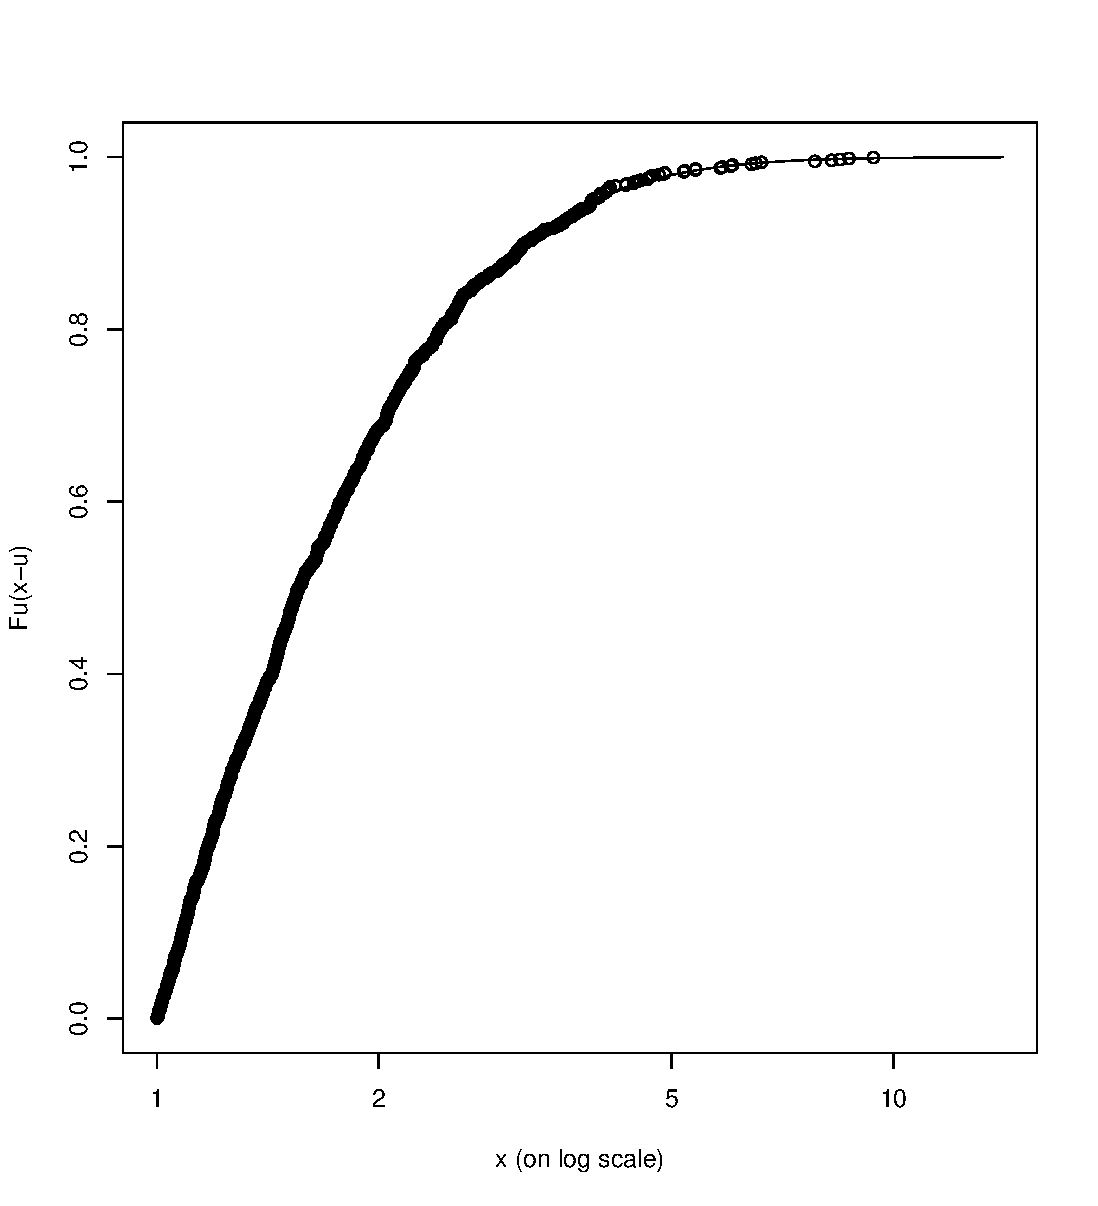
\includegraphics[width=0.6\linewidth]{C:/Users/Rikard/OneDrive/Statistik 2020-2021/Statistik C/Examensarbete/Extreme Value Theory/RmarkdownUppsaladown/index/omxs30emp} 

}

\caption{Empirical distribution of excesses and fitted GPD for the OMXS30 percentage loss data.}\label{fig:empomxs30}
\end{figure}
\begin{figure}[H]

{\centering 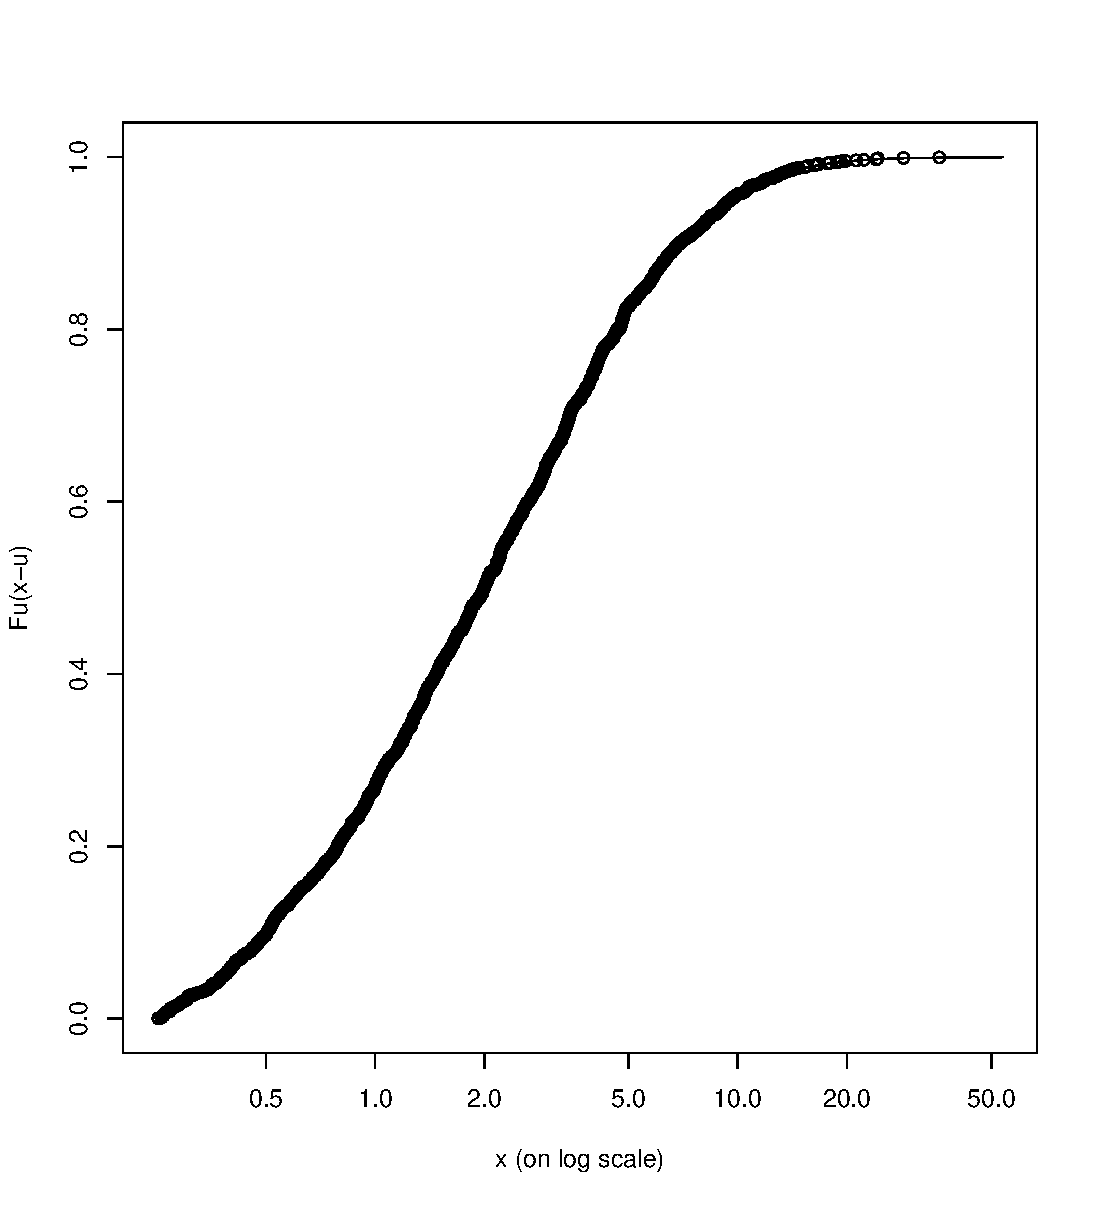
\includegraphics[width=0.6\linewidth]{C:/Users/Rikard/OneDrive/Statistik 2020-2021/Statistik C/Examensarbete/Extreme Value Theory/RmarkdownUppsaladown/index/bitcoinemp} 

}

\caption{Empirical distribution of excesses and fitted GPD for the Bitcoin percentage loss data.}\label{fig:empbitcoin}
\end{figure}
\begin{figure}[H]

{\centering 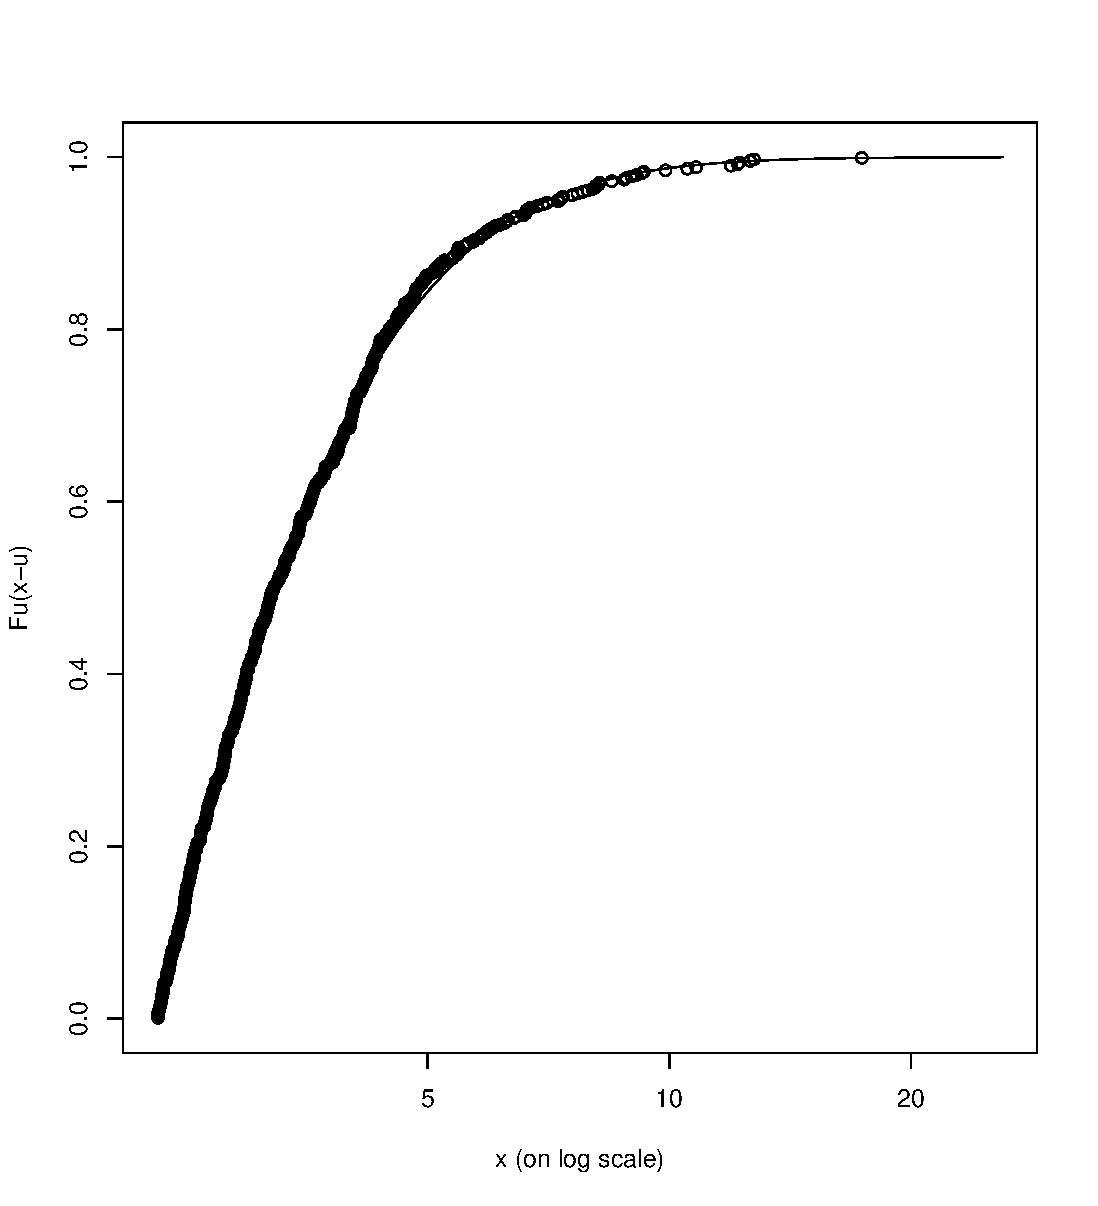
\includegraphics[width=0.6\linewidth]{C:/Users/Rikard/OneDrive/Statistik 2020-2021/Statistik C/Examensarbete/Extreme Value Theory/RmarkdownUppsaladown/index/brentemp} 

}

\caption{Empirical distribution of excesses and fitted GPD for the Brent crude percentage loss data.}\label{fig:empbrent}
\end{figure}
\begin{figure}[H]

{\centering 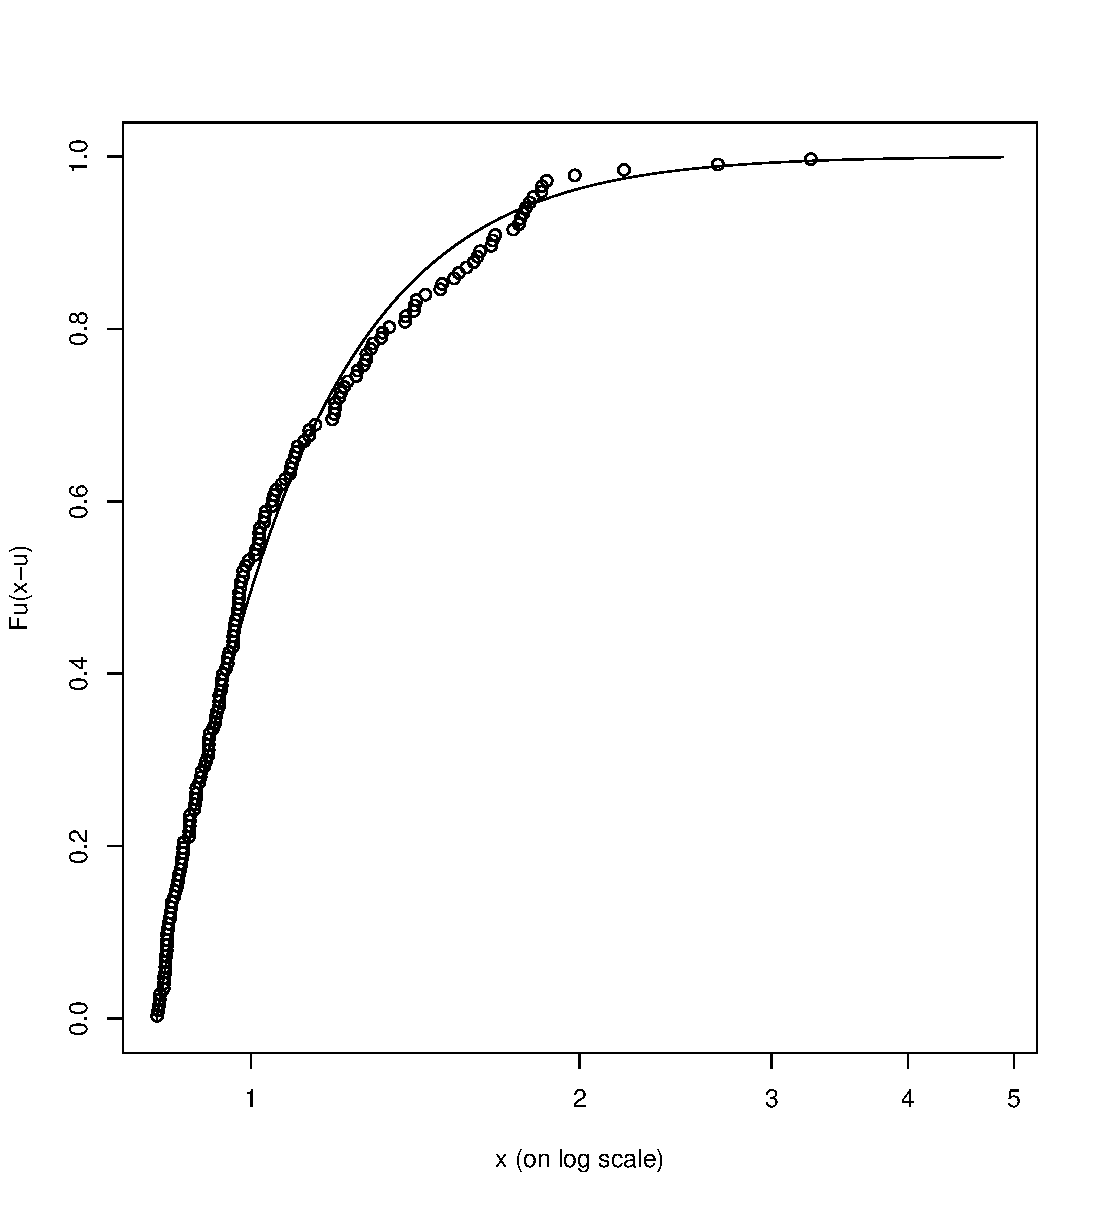
\includegraphics[width=0.6\linewidth]{C:/Users/Rikard/OneDrive/Statistik 2020-2021/Statistik C/Examensarbete/Extreme Value Theory/RmarkdownUppsaladown/index/sekemp} 

}

\caption{Empirical distribution of excesses and fitted GPD for the SEK/EUR percentage loss data.}\label{fig:empsek}
\end{figure}
\begin{figure}[H]

{\centering 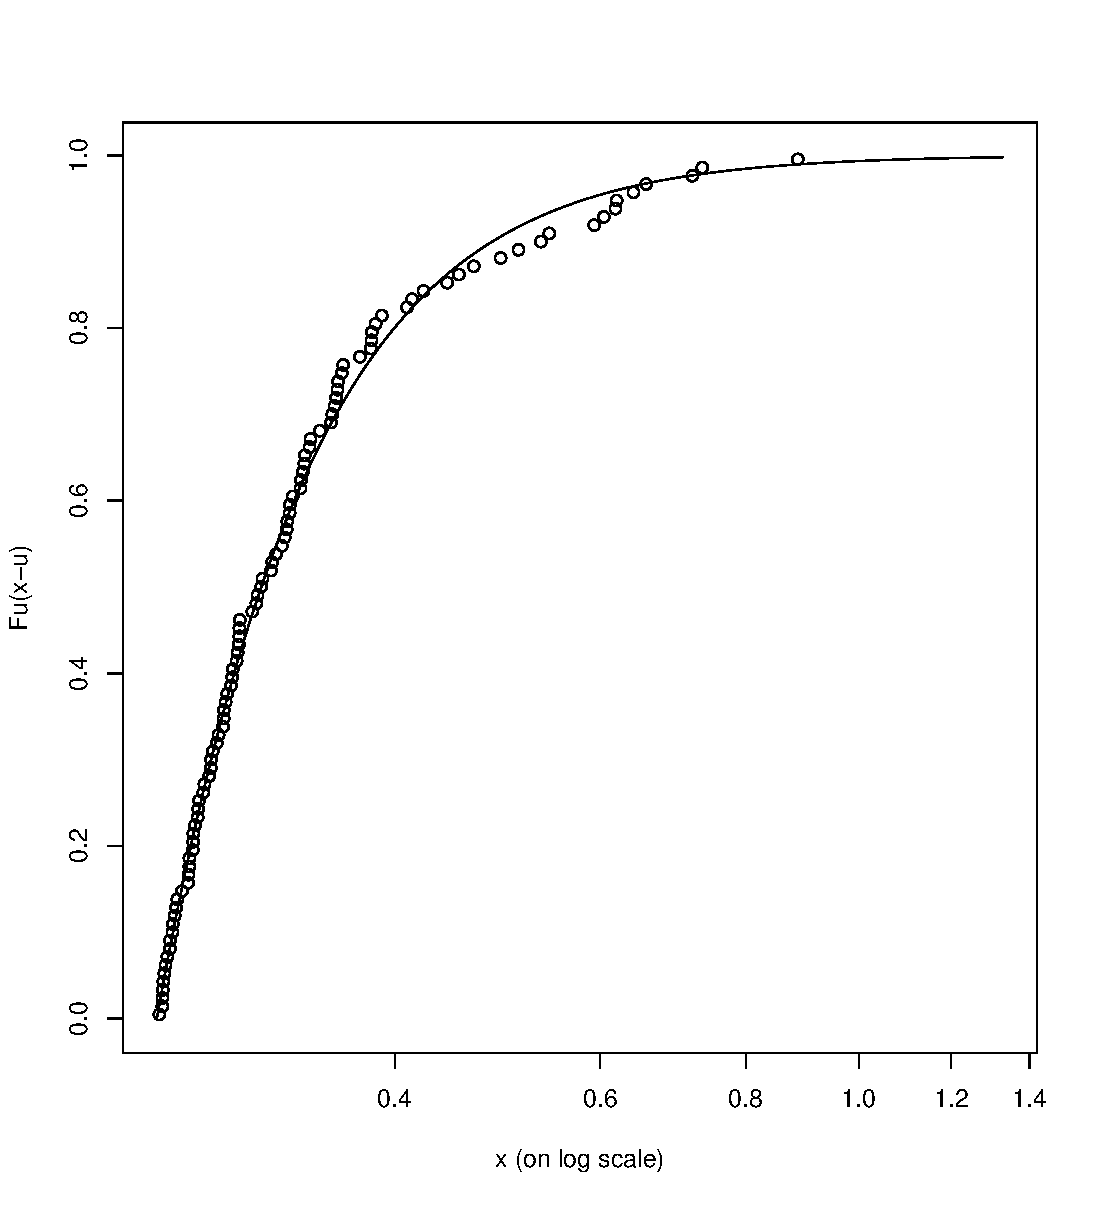
\includegraphics[width=0.6\linewidth]{C:/Users/Rikard/OneDrive/Statistik 2020-2021/Statistik C/Examensarbete/Extreme Value Theory/RmarkdownUppsaladown/index/treasuryemp} 

}

\caption{Empirical distribution of excesses and fitted GPD for the OMRXBOND percentage loss data.}\label{fig:emptreasury}
\end{figure}
\hypertarget{sec:tailprobabilities}{%
\subsubsection{Estimated tail probabilities}\label{sec:tailprobabilities}}
\begin{figure}[H]

{\centering \includegraphics[width=0.8\linewidth]{thesis_files/figure-latex/omxs30rmplot-1} 

}

\caption{Estimated tail of the OMXS30 percentage loss data with points plotted at empirical tail probabilities from the empirical distribution function.}\label{fig:omxs30rmplot}
\end{figure}
\begin{figure}[H]

{\centering \includegraphics[width=0.8\linewidth]{thesis_files/figure-latex/bitcoinrmplot-1} 

}

\caption{Estimated tail of the Bitcoin percentage loss data with points plotted at empirical tail probabilities from the empirical distribution function.}\label{fig:bitcoinrmplot}
\end{figure}
\begin{figure}[H]

{\centering \includegraphics[width=0.8\linewidth]{thesis_files/figure-latex/brentrmplot-1} 

}

\caption{Estimated tail of the Brent crude percentage loss data with points plotted at empirical tail probabilities from the empirical distribution function.}\label{fig:brentrmplot}
\end{figure}
\begin{figure}[H]

{\centering \includegraphics[width=0.8\linewidth]{thesis_files/figure-latex/sekrmplot-1} 

}

\caption{Estimated tail of the SEK/EUR percentage loss data with points plotted at empirical tail probabilities from the empirical distribution function.}\label{fig:sekrmplot}
\end{figure}
\begin{figure}[H]

{\centering \includegraphics[width=0.8\linewidth]{thesis_files/figure-latex/treasuryrmplot-1} 

}

\caption{Estimated tail of the OMRXBOND percentage loss data with points plotted at empirical tail probabilities from the empirical distribution function.}\label{fig:treasuryrmplot}
\end{figure}
% change rmd_files in `_bookdown.yml` files to determine order
% note that references and appendix are also contained here.


\end{document}
